\documentclass[12pt,preprint]{aastex}



%%% PACKAGES %%%%%%%%%%%%%%%%%%%%%%%%%%%%%%%%%%%%%%%%%%%%%%%%%%%%%%%%%%%%%%%%%%%

\usepackage{amsmath}
\usepackage{xspace}   % fixes spaces after custom commands
\usepackage{float}    % exact placement of figures (using \begin{figure}[H])
%\usepackage{caption}  % better captions for floats
\usepackage{color}  % well... color...
%\usepackage{todonotes}  % only used during writing..
%\usepackage{ifdraft}    % executes commands if in draft mode
\usepackage{setspace}    % remove this pgk for final compile!! 
\usepackage{subfigure}

\usepackage{longtable}   % those two to generate the 2 ol table
\usepackage{multicol}

%%% DEFINITIONS %%%%%%%%%%%%%%%%%%%%%%%%%%%%%%%%%%%%%%%%%%%%%%%%%%%%%%%%%%%%%%%%

\def\half{{\textstyle\frac12}}
% makes it easier to have consistent writing, and easy change if needed
\newcommand{\spl}{SpaghettiLens\xspace}
\newcommand{\sw}{SpaceWarps\xspace}
\newcommand{\tEr}{Einstein radius\xspace}
\newcommand{\gEr}[1][]{$\Theta_\text{E#1}$\xspace}
\newcommand{\kenc}[1][r]{$\kappa_\text{encl}(#1)$\xspace}
\newcommand{\kap}[1][r]{$\kappa(#1)$\xspace}


% shorcuts for refs
\newcommand{\figref}[1]{figure~\ref{fig:#1}}
\newcommand{\secref}[1]{section~\ref{sec:#1}}
\newcommand{\tabref}[1]{table~\ref{tab:#1}}
\newcommand{\Figref}[1]{Figure~\ref{fig:#1}}
\newcommand{\Secref}[1]{Section~\ref{sec:#1}}
\newcommand{\Tabref}[1]{Table~\ref{tab:#1}}


% todo annotations on side in red. easy to search for at the end
\newcommand{\todo}[2][red]{%\marginpar{\raggedright\scriptsize\sffamily\textcolor{red}{#1}}}
%{\marginpar{\raggedright\sffamily\textcolor{red}\footnotesize
%\setstretch{1.025}%
%#1}}}
\textcolor{#1}{\textbullet}%
\marginpar{\colorbox{#1}{\parbox{\marginparwidth}{%
\setstretch{0.4}\sffamily\textcolor{black}{\scriptsize{#2}}}}}}

\newcommand{\needfig}[1][]{%
\colorbox{yellow}{\parbox{0.5\textwidth}{%
\vspace{0.5cm}\setstretch{0.5}\textcolor{black}{\scriptsize{fig #1}}\vspace{0.5cm}}}%
\marginpar{\colorbox{yellow}{\parbox{\marginparwidth}{%
\setstretch{0.4}\sffamily\textcolor{black}{\scriptsize{fig}}}}}}

\setlength{\marginparsep}{0mm}
\setlength{\marginparwidth}{2.2cm}

% quick todo annotations
%\newcommand{\todocit}{\todo{insert citation}}
%\newcommand{\todoref}{\todo{insert ref}}
%\newcommand{\todochk}{\todo{check again}}
\newcommand{\needcite}[1][]{\todo[green]{cit #1}}
\newcommand{\needref}[1][]{\todo[cyan]{ref #1}}
\newcommand{\needchk}[1][]{\todo[red]{chk #1}}

% using todo notes:
%\newcommand{\needcite}[1][]{\todo[color=blue!40, size=\tiny]{cit: #1}}
%\newcommand{\needref}[1][]{\todo[color=green!40, size=\tiny]{ref: #1}}
%\newcommand{\needchk}[1][]{\todo[color=yellow!40, size=\tiny]{chk: #1}}
%\newcommand{\needfig}[1][]{\missingfigure{#1}}



\newcommand{\hr}{\vspace{5mm}\noindent\rule{0.8\textwidth}{0.4pt}\vspace{5mm}}




%%% DOCUMENT %%%%%%%%%%%%%%%%%%%%%%%%%%%%%%%%%%%%%%%%%%%%%%%%%%%%%%%%%%%%%%%%%%%

\begin{document}


\title{Lens Modeling in \sw}
\author{First Author,\altaffilmark{1}
Second Author,\altaffilmark{2} and
Third Author\altaffilmark{3}}
\altaffiltext{1}{First place}
\altaffiltext{2}{Second place}
\altaffiltext{3}{Third place}


\begin{abstract}
In Spacewarps, volunteers are invited to search sky surveys for lens
candidates.  Here we report on a system that allows experienced
volunteers to model lens candidates.  A sample of 29 simulated lenses
were modelled, each multiple times.  The quality of the models was
then examined in two ways.  First, the image parities and time
orderings: these were identified correctly in most cases, but not
always.  Second, the mean convergence (equivalent to the enclosed
mass): this was constrained consistently well in the image region.
The performance of professionals and experienced volunteers was
comparable.
\end{abstract}

\keywords{}
\section{Introduction}


Gravitational lenses (GLs), predicted by ART, can be used as a tool by astronomers to examine many properties of the cosmos.
They allow for example to estimate the masses and their distribution of galaxies, automatically including the hard to grasp dark matter.
Further more, they allow an estimate on cosmological parameters like the Hubble constant \citep{Saha2006} and the mass density \needcite.

%To accheve this, one needs to find / identify lenses and in a second step model those lenses to get involved parameters.

How to find gravitational lenses? Huge amount of image data from surveys that needs to be processed.
Even more comming in the future with new surveys \needcite
Robotic procession has been suggested \needcite, and tested \needcite, but has failed so far to be convincing \needcite.
Another suggestion involves humans, volountiers \footnote{A volounteer is considered everybody that has no background in astro physics.}.
\sw uses this approach with great succes so far.\needcite


Next step involves modeling. that needs advanced knolegde and takes a lot of time.
Too much time to be done by astronomers them selves as the results from new surveys and identifiers like \sw come in.
So there is a demand of a means to modell a great amount of identified lens data, that scales with increasing data amount.


The purpose of this study was to provide a means to model a large amount of gravitational lenses by showing that gravitational lens modelling can be learned / done by volunteers.
We suggest, that volunteers will be as successful as professionals with modelling if provided with an easy to use tool with visual feedback (WYSIWYG) and a minimal set of instructions.
Voulnteers will then croud work (using buzz word here ;) ) / work collarobartive on modelling lenses from several sources / groups at a central place.
Since this is a iterative learning process, the more involved volunteers will quickly gain knoledge that can be passed down to new volunteers.
That creates a social structre that scales well with the number of volunteers, as other projects\needcite have already shown.
Finding people working as volunteers has been shown to be successful lst but not least by \sw and the whole galaxy zoo project.
To test the peoples abilities, we invesigated the performance of a first set of volunteers modelling a set of simulated lenses.
We tested the ability to correcly identify lensed images and reproduce simmilar mass maps of the lens.

\section{Fermat's Principle} \label{sec:Fermat}

Explain Fermat's principle
\begin{equation}
\hbox{arrival time} = A_{\rm geom} - A_{\rm grav}
\end{equation}
By convention, $A_{\rm grav}$ is defined in such a way that it is
negative, hence the minus sign.

Although $A_{\rm geom}$ and $A_{\rm grav}$ are times, we are going to
write them as if they are areas.  In other words, we will suppress a
constant factor in the $A$.  That factor is basically the lens
distance times the speed of light, but the precise expression is given
in the Appendix.

Introduce the Laplacian $\nabla^2 f(x,y)$ is
\begin{equation}
 \frac{ f(x+\Delta x, y) + f(x-\Delta x, y) +
        f(x, y+\Delta y) + f(x, y-\Delta y) - 4 f(x,y) }
      {\Delta x \; \Delta y}
\end{equation}
in the limit of $\Delta x,\Delta y$ small.

Let $x,y$ be coordinates on the lens, transverse to the line of sight.
Let there be a point source behind $x=0,y=0$.  Then
\begin{equation}
A_{\rm geom}(x,y) = \half(x^2 + y^2)
\end{equation}
\begin{equation}
\nabla^2 A_{\rm grav}(x,y) = 2\kappa(x,y)
\end{equation}
Here $\kappa$ is a dimensionless quantity with two distinct physical
interpretations.  On the one hand, it is the sky projected density ---
in special units, to make it dimensionless.  On the other hand,
$\kappa$ is the {\em convergence\/} of a bundle of rays.
\begin{figure}
  \centering
  \subfigure{\includegraphics[width=0.45\textwidth]
             {fig/sims/006941/input.png}} \\
  \subfigure{\includegraphics[width=0.45\textwidth]
             {fig/sims/007022/input.png}} \\
  \subfigure{\includegraphics[width=0.45\textwidth]
             {fig/sims/006919/input.png}}
  \caption{Examples of Spaghetti input.  The models from these appear
    later in Figures \ref{fig:6941}, \ref{fig:7022} and \ref{fig:6919}.
  \label{fig:input-spag}}
\end{figure}

\subsection{\spl} \label{sec:SpaghettiLens}

A saddle point is recognizable in a contour map because contours do
not loop around it, they tend to approach and then pull away.  There
is one contour ---the saddle-point contour--- that makes an X on the
saddle point itself.  A saddle point contour may not appear on a plot
(and Figure~\ref{fig:arriv} does not show one.  But we can tell from
the other contours where the saddle-point contour would be.



Give a guess for the maximum, minimum and saddle points.  Program
tries find $\kappa(x,y)$ that reproduces these properties exactly, and
looks reasonably like a galaxy.  Solution not unique, an ensemble
generated.

\hr

SpaghettiLens is build on top of GLASS \citep{Lubini2012}, that builds and improves upon PixeLens \citep{Saha2004}.
It provides a web based graphical user interface that allows to trace contours with the mouse and identify extremal points by clicking on the image.
\spl then tries to find a mass distribution $\kappa(x,y)$ that reproduces the input parameters.
Since there is no unique solution, \spl samples the solution space and produces an ensemble of solutions, as described in the paper \citep{Lubini2012}.
It provides direct visual feedback by rendering a synthetic image side by side the original image, such that users can directly compare the predictions of their model to the survey image.
It additinally provides plots of the modelled mass distribution and the contour lines of arrival time surface as feedback. 

Using this direct visual feedback, even unexperienced users can successfully model lenses using a iterative approach if they know what to look for.

The modelling process consitis of three basic steps:

\begin{enumerate}
  \item identify lensed images and separate them from other background light sources
  \item classify and order images accoring to arrival time. (local minima, maxima, saddlepoints)
  \item fine tune the arrangement, identify addidional external point masses influencing the result
\end{enumerate}

\spl assists volunteers with several features in this process.
Step 1 by supplying several images from several bands (not yet implemented in \sw).
Step 2 by restricting the user, only valid configuration can be entered, the odd number theorem\needcite is taken care of.
Step 3 by providing the visual feedback. Users can check the generated mass distribution and synthetic image.

Explanation:
Synthetic image: A rendering of the derivative of the arrival time for each pixel. This leads to a black and white image that reasonably looks like the visual appearace of the model.

Volunteers enter an assumed lens configuration and get a rendered synthetic image along with a reconstructed / simulated mass map and reconstructed / simulated contour lines.
This allows volunteers to directly see the effect of changing the parameters of the model and to iteratively approach a good solution.

In the next step, several volunteers can work together / exchange their ideas and models and try to improve previous modelling attempts by others.
This leads to a set of models organised in a branching, tree like structre for each model.
Volunteers then organise them selves to narrow down the different branches and come up with a few consensus models in the end.

\spl provides plug ins to support any data source. At the moment, a data link to \sw and to the MasterLens database\needcite are implemented.







\section{A lens modeling challenge} \label{sec:results}

% \subsection{\sw} \label{sec:SpaceWarps} some words about \sw

Interested volunteers from the \sw forum were initially introduced to
\spl through a video tutorial and by videocon.  After this
introductory stage, a modelling challenge was presented.  This
consisted of 29 simulated lenses (sims) covering a range of lensing
configurations.

\subsection{The simulated lenses} \label{sec:sims}

The sims were generated by AM, in consultation with PM and AV.  In the
interest of blind testing, the information in this section was
revealed neither to RK, while choosing the challenge set, nor to the
people making models (EB, CC, CM, JO, PS and JW) until they were done.

The sims produced using {\tt gravlens}
\citep{2001astro.ph..2341K,2001astro.ph..2340K} and were of three
kinds, as follows.

\begin{itemize}
  \item {\em Quasar:\/} A singular elliptical isothermal plus constant
    external shear, with a circular Gaussian source.
  \item {\em Galaxy:\/} Lens as with quasar, but elliptical de
    Vaucouleurs source.
  \item {\em Galaxy:\/} Lens is circular NFW plus one dominant
    elliptical SIE and perturbating elliptical SIEs, source as with
    galaxy.
\end{itemize}

Singular isothermal is in equations (33-35) of
\cite{2001astro.ph..2341K} with core radius set to zero. NFW is
equations (48,50) of the same paper, and shear is the $\gamma$ term in
equation (76) of that work.

\subsection{Some example models}

Figure \ref{fig:6941} shows a simple example.

Figure \ref{fig:6975} shows an example where substructure introduces a
complication, but model ok.

Figure \ref{fig:6937} shows a case where substructure leads to a
poorer model.

Figure \ref{fig:6975} shows a nice symmetric quad.

Figure \ref{fig:6990} shows a long-axis quad.

Figure \ref{fig:6919} shows a short-axis quad.

Figure \ref{fig:6915} shows an inclined quad.

Figure \ref{fig:6971} shows incorrect identification, but the enclosed
mass still quite well recovered.


\subsection{The test setup} \label{sec:testsetup}

To estimate the performance of the volunteers and the quality of the generated models, two test T1 and T2 were done.
%\begin{enumerate}
%  \item (T1) Correct identification of extremal points
%  \item (T2) Reproduction of the mass distribution of the lens
%\end{enumerate}

T1 tested the volunteers ability to reconstruct the arrival time surface given a survey image containing a sim.
This task consists of two parts.
First, the correct identification and location of lensed images (T1a).
Second to find the correct ordering in respect of the arrival time for the identified lensed images (T1b).

While we expected T1a to be trivial, given the nature of the survey images and the success of \sw, we expect T1b to pose more problems.
T1b tests the volunteers understandings of the theory of arrival time surfaces and the odd number theorem.
While we can provide the volunteers with some general rule of thumbs, T1b involves a lot of imagination and guessing and therefore a training effect could be visible in this test.

T1 was also designed to give some feedback on the difficulties volunteers encounter, to further imrove the tutorial materials.

The second test T2 was to compare the desired results of a modeling process, the mass distribution of the lens $\kappa(x, y)$.
To get a means of comparing the simulated data (sims) to the generated modeled data (models), the total convergence, also called enclosed mass $\kappa_{\text{encl}}(r)$ for both was calculated.
The Einstein radius $\Theta_E$ is defined by $\kappa_{\text{encl}}(\Theta_E)=1$ and gives a number that allows the comparison between the sims and the models.

\todo{!} Should I write down prior expectation for T2 too?




\subsection{First test T1} \label{sec:tests.t1}

The evaluation of the volunteers performance for T1 was done manually, comparing their input from \spl and the resulting reconstructed arrival time surface contour line plot (arrival plot) to the arrival plot genreated using simulation parameters.
\Figref{output_compare} shows the setup used to evaluate the models.

\begin{figure}
  \centering
  \subfigure{\includegraphics[width=0.45\textwidth]
             {fig/sims/006917/input.png}}
  \subfigure{\includegraphics[width=0.45\textwidth]
             {fig/sims/006917/spaghetti.png}} \\
  \subfigure{\includegraphics[width=0.45\textwidth]
             {fig/sims/ASW0001hpf/arriv.png}}
%  \subfigure{\includegraphics[width=0.45\textwidth]
%             {fig/sims/ASW0001hpf/extr_points.png}}
  \caption{Examples of Spaghetti input (left top) and modeled arrival time surface (right top) vs reconstructed arrival time surface from simulation parameters (bottom left), additionally using a extremal point detector (bottom right).
  \label{fig:output_compare}}
\end{figure}

To evaluate T1a and T1b, each model was evaluated with two binary tests.
The first is passed, if all the images have been identified and are approx. within $\pm0.05\cdot\text{imgwidth}$.
The second test is passed, if those identified points have the right parity, ordering with respect to arrival time.

Additionally, ten types of errors that could occur were analyzed, where each model could contain multiple of those.
The complete table with the results for each model can be found in the appendix, \tabref{detail_results}.

In \tabref{stats} a summary of this evaluation is presented.

%\begin{enumerate}
%1  \item inaccurate placement in an extended arc
%2  \item wrongly identified sad and min in 3 image configuration
%3  \item identified only 3 instead of 5 images
%4  \item tried to model an arc with a min instead of min-sad-min
%5  \item PI-err (rotation by 180 degrees; in 5 image configuration, exchanged the ordering of the two saddle points)
%6  \item PI/2-err (rotation by 90 degree; sad$\longmapsto$min$\longmapsto$sad$\longmapsto$min$\longmapsto$sad)
%7  \item missed faint image(s)
%8  \item tried to model an arc with min-sad-min instead of only min
%9  \item did identify two close by images as one
%10  \item used 7 or more image to model a 5 image system.
%\end{enumerate}

\input{tab/auto/_stats}


We conclude that the volunteers are performing very well identifying and positioning images (T1a), with a performance of 92\% (approxPlace p=0.92).
Most of the problems where due to unclear arc-like structures (Error 1, p=0.18; Error 4, p=0.03; Error 8, p=0.04).
Critical failures like the failure to identify all fife images in an fife image system (Error 3, p=0.04) or to include too many images (Error 10, p=0.01) did almost never happened.
From this we conclude that the introduction materials was adequate and the volunteers understand the basics of gravitational lensing.

\todo{add more detail?} Add more details like total amount of images detected / tot am images (rightPlace fraction)??

The assignment of the parity of the images (T1b) posed a more difficult task.
In 59\% (rightOrder, p=0.59, N=70) of the cases the volunteers succeeded to identify the right configuration.
Most of the failures are due to Error 6 (PI/2), with N=38, p=32\%, followed by Error 5 (PI) with N=7, p=6\%.
For an example of type 6 error, see \figref{6971}.
While these errors occurred, we suspect they can be avoided with better training material and some examples for the obvious cases.
For more challenging cases, like very symmetrical distribution of the lensed images (for example model 6971, \figref{6971}), those errors should still produce plausible results, as will be explained in the next section.







\subsection{Second test T2} \label{sec:results.2}

To compare the enclosed mass profile and the Einstein radius of the simulation and the models, \kenc was calculated using the mass map \kap[x,y] directly generated in the modeling process.
From the ensemble of models generated by one modelling process, the mean is taken as the resulting $\kappa(r)$ to calculate $\theta_E$.
To estimate the errors, also the extremal models are used to estimate a lower and upper limit for $\theta_E$.
These results can be seen in \figref{eR_all_models}.
This figure shows that this tecnique of esitmating the error is underestimating the error significantly and should be improved for further analysis.

\begin{figure}[htbp]
  \centering
    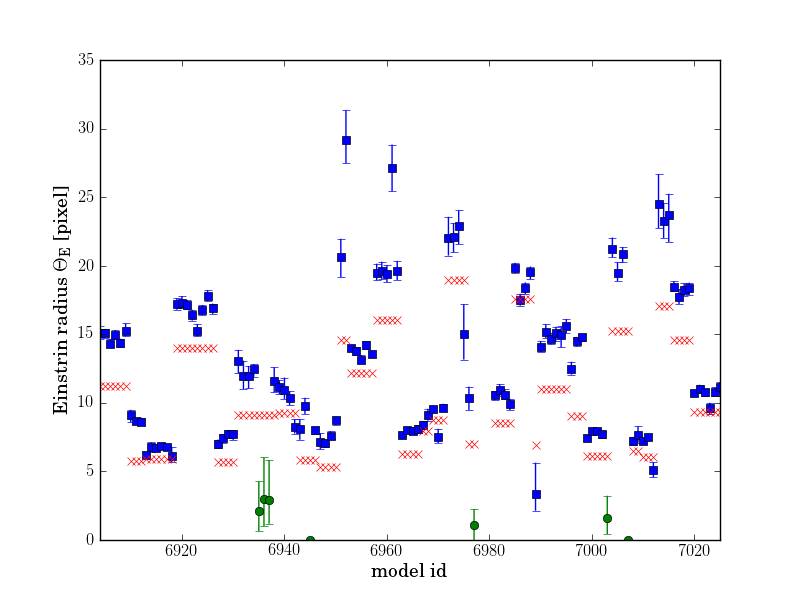
\includegraphics[width=0.80\textwidth]{fig/sims/eR_1.png}
  \caption{\tEr \gEr for all models with estimated erros in blue, \gEr of simulation in red}
  \label{fig:eR_all_models}
\end{figure}

In \figref{eR_per_sim} can be seen, that the calculated \tEr \gEr of the models tend to be too high.
The overshoot varies from around 0.2 to 0.4 for for good models.
One of the reasons for this is, that it's hard to get the center of the lens on spot.
An offset leads to a a flatter mass profile for the model compared to the simulation.



\begin{figure}[htbp]
  \centering
    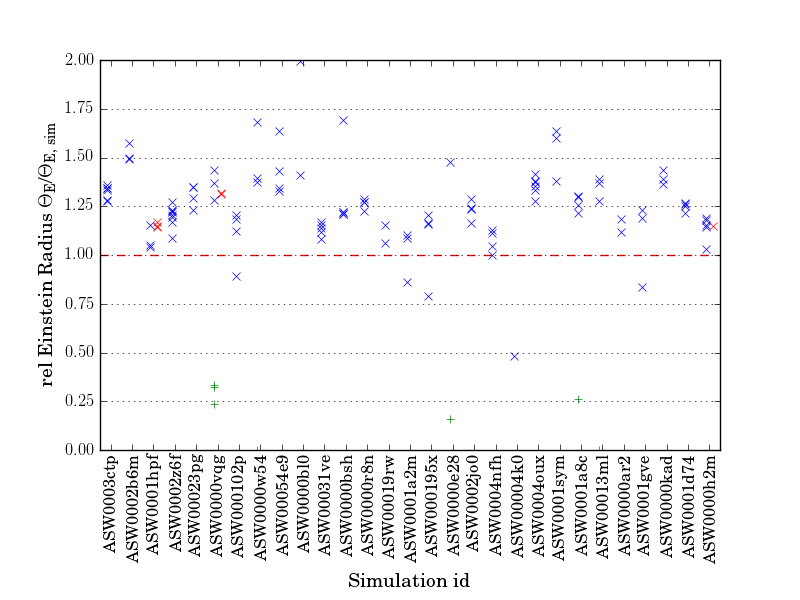
\includegraphics[width=0.80\textwidth]{fig/sims/eR_4.png}
  \caption{relative Einstein Radius for each model, per sim. }
  \label{fig:eR_per_sim}
\end{figure}


Error 5 and 6 happen mostly in very symmetric images, where it's hard to tell
It changes the orientation of the mass distribution \kap[x,y].
But \kenc and thus the \tEr \gEr is not changed, and thus the final result is still a valid model.
This can be easily corrected, if further analysis is done for the modeled system and time delays are known.




\clearpage

\section{Extensions needed} \label{sec:todo}

As seen in \secref{tests.t1}, volunteers fail mostly in two situations:
when to identify an arclike structure while placing the points
and in 5 image configurations, that are quite symmetric, then to identify the correct ordering of the points.

The first can be improved by additional images from different filters (?)
Will be implemented with a next major \spl upgrade.

The second can be made less by better training (introduce the ruler), may be more filters help too?

We hope that those problems are also taken care of when staring collaborative modeling. (Already in progress)
Basics are available ('revise functionality') but better community tools would help (having overview, comparison between different models ect...)

Lenses with more than one maximum can be allowed for.  See Figure 5c
in \citep{2001ApJ...557..594R} and Figure 4b in
\cite{2003ApJ...590...39K}.

Supply several images from several bands.



\clearpage

\appendix

\section{More on Lensing Theory} \label{sec:more-theory}

In \secref{Fermat}, for the sake of a more intuitive
explanation, we suppressed some constant factors in
equations \eqref{eq:Ageom}, \eqref{eq:Ageom} and \eqref{eq:Poisson}.
Here we fill in the details.

First we define comoving distances.
\begin{equation}
\int \frac{dz}{\sqrt{\Omega_m(1+z)^3 + \Omega_\Lambda}}
\end{equation}
\begin{equation}
\begin{aligned}
&D_S    &                                &\int_0^{a_S} \\
\noalign{\medskip}
&D_{LS} & = \frac c{H_0} \ \times \quad  &\int_{z_L}^{z_S} \\
\noalign{\medskip}
&D_L    &                                &\int_0^{z_L}
\end{aligned}
\end{equation}
Can replace comoving distances $D$ with angular-diameter distances
$d$, and so on:
\begin{equation}
\begin{aligned}
D_S &= (1+z_S) \, d_S \\
D_{LS} &= \frac{1+z_S}{1+z_L} \, d_{LS} \\
D_L &= (1+z_L) \, d_L
\end{aligned}
\end{equation}
Angular-diameter distances are always smaller than comoving distances.
Locations on the lens plane can be replaced angular coordinates on the
sky, as
\begin{equation}
(x,y) = d_L (\theta_x,\theta_y) \,.
\end{equation}

The $A$ times and the $\kappa$ density are related to physical arrival
time $t$ and density $\Sigma$ as
\begin{equation}
\begin{aligned}
A           &= \frac{cD_L}{(1+z_L)^2} \frac{D_{LS}}{D_S} \times t \\
\kappa(x,y) &= \frac{4\pi G}{c^2} \frac{D_L}{1+z_L} \frac{D_{LS}}{D_S}
               \times \Sigma(x,y)
\end{aligned}
\end{equation}
Letting the source be behind $(s_x,s_y)$ rather than behind the
origin, we have
\begin{equation}
\begin{aligned}
t_{\rm geom} &= \frac{(1+z_L)^2}{2cD_L} \frac{D_S}{D_{LS}}
\left( (x-s_x)^2 + (y-s_y)^2 \right)
\nabla^2 t_{\rm grav} &= -(1+z_L)\frac{8\pi G}{c^3} \, \Sigma(x,y)
\end{aligned}
\end{equation}
We can now compare with equations (2.1) to (2.6)
from \cite{1986ApJ...310..568B}.



\clearpage
\newpage

\bibliographystyle{apj}
\bibliography{bib/ms}

\newpage

\begin{figure}
\centering
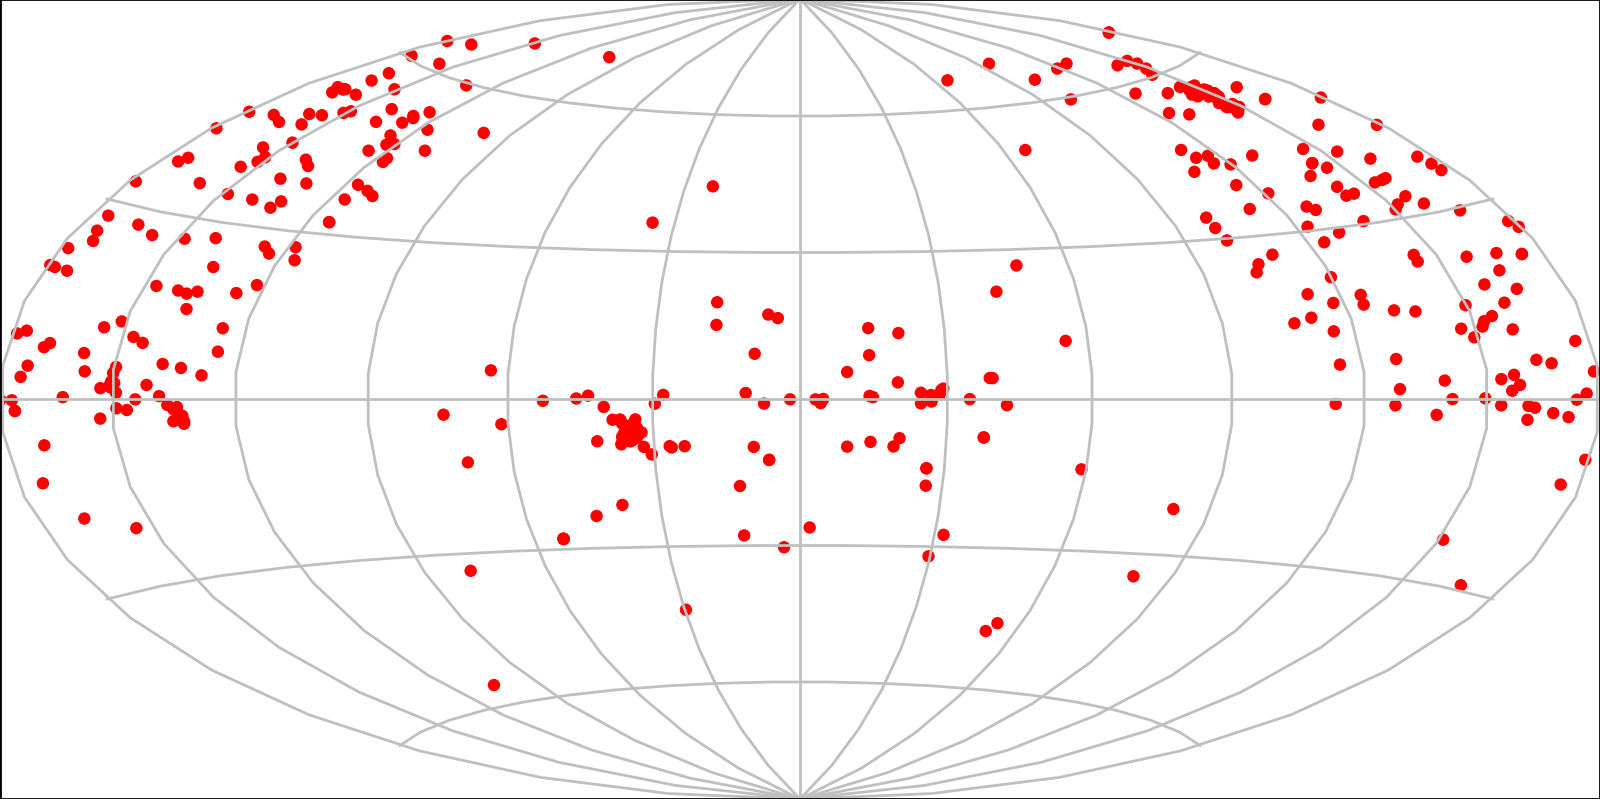
\includegraphics[width=.4\vsize]{fig/lenssky.png}
\caption{Sky distribution of 398 published lenses considered secure as
  of September 2013 (from the Masterlens catalog at the University of
  Utah, maintained by Joel Brownstein and Leonidas Moustakas.) The map
  is in Hammer-Aitoff projection, with North up and $\rm RA=0$ in the
  middle.  The empty swathes to the left and right of center are the
  Milky Way.}
\label{fig:masterlens}
\end{figure}

\begin{figure}
\centering
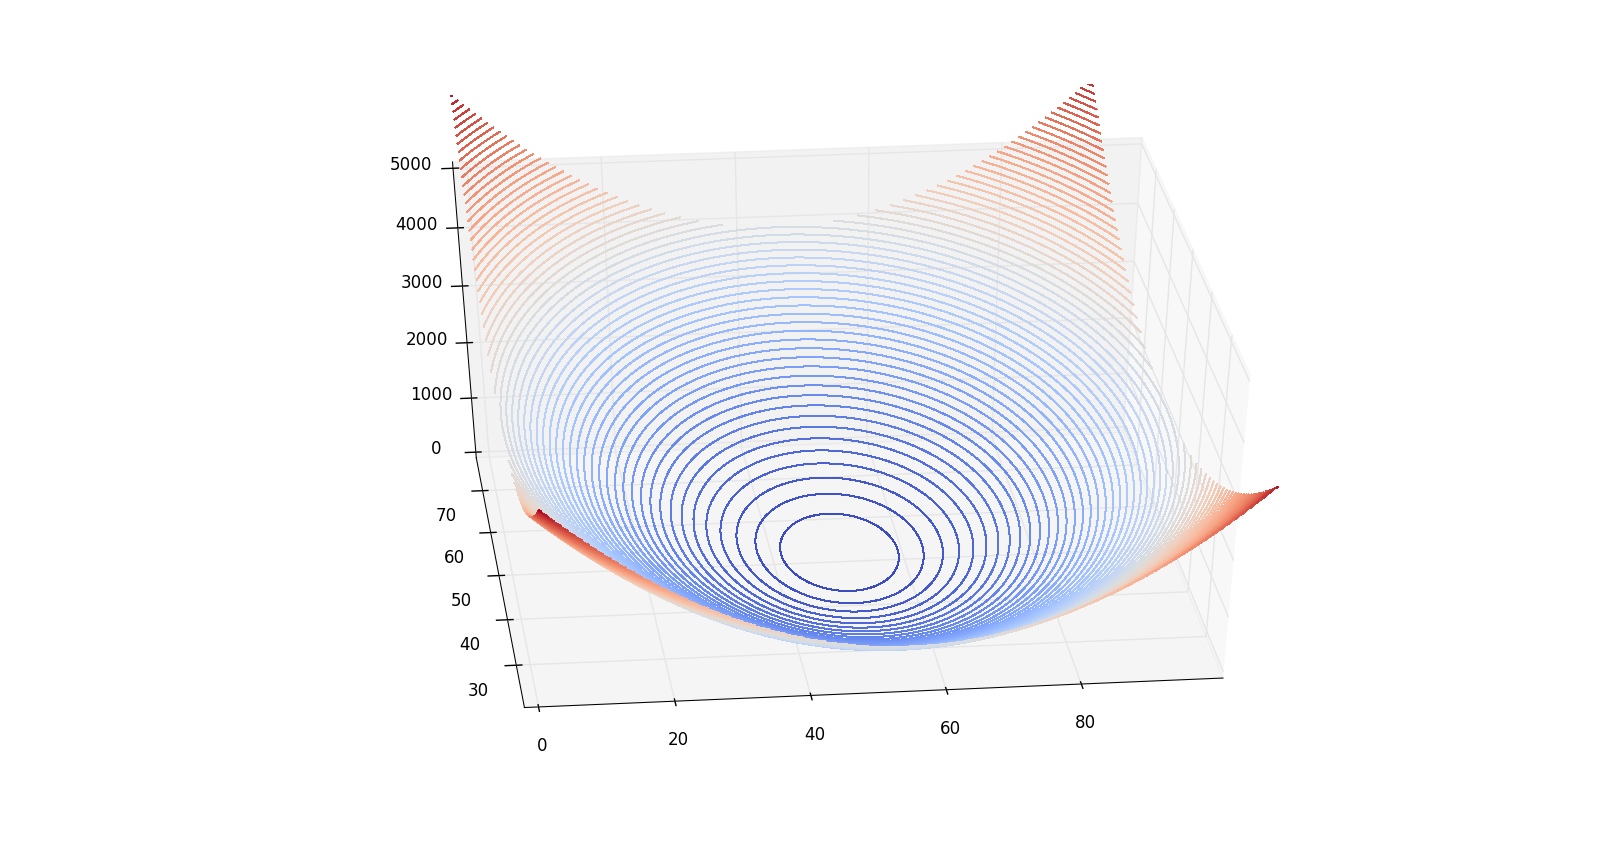
\includegraphics[height=.3\vsize]{fig/arriv1.png}
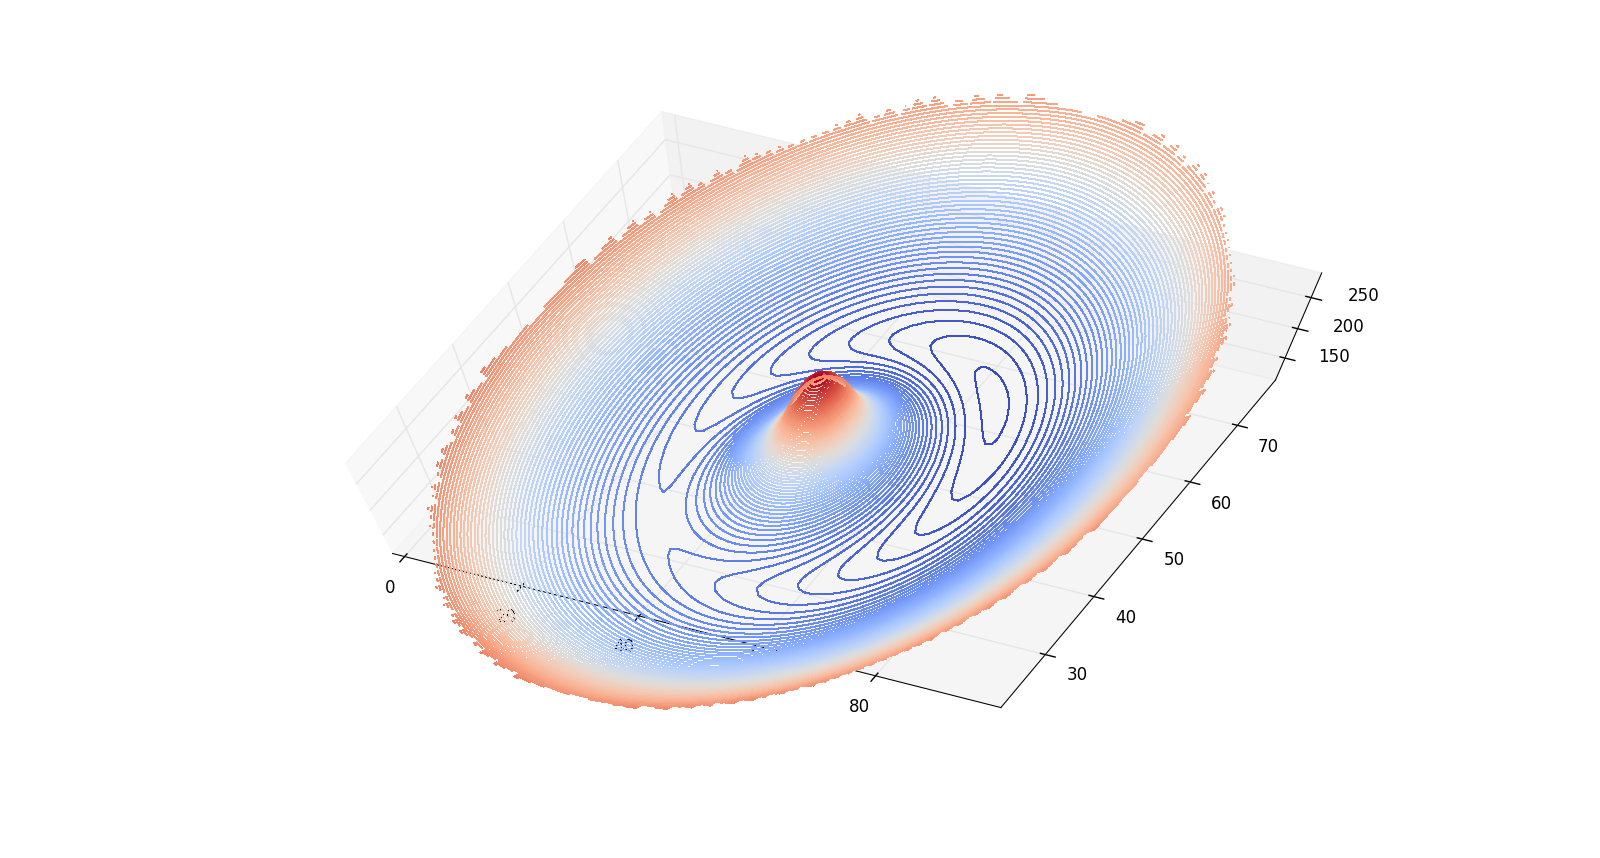
\includegraphics[height=.3\vsize]{fig/arriv2.png}
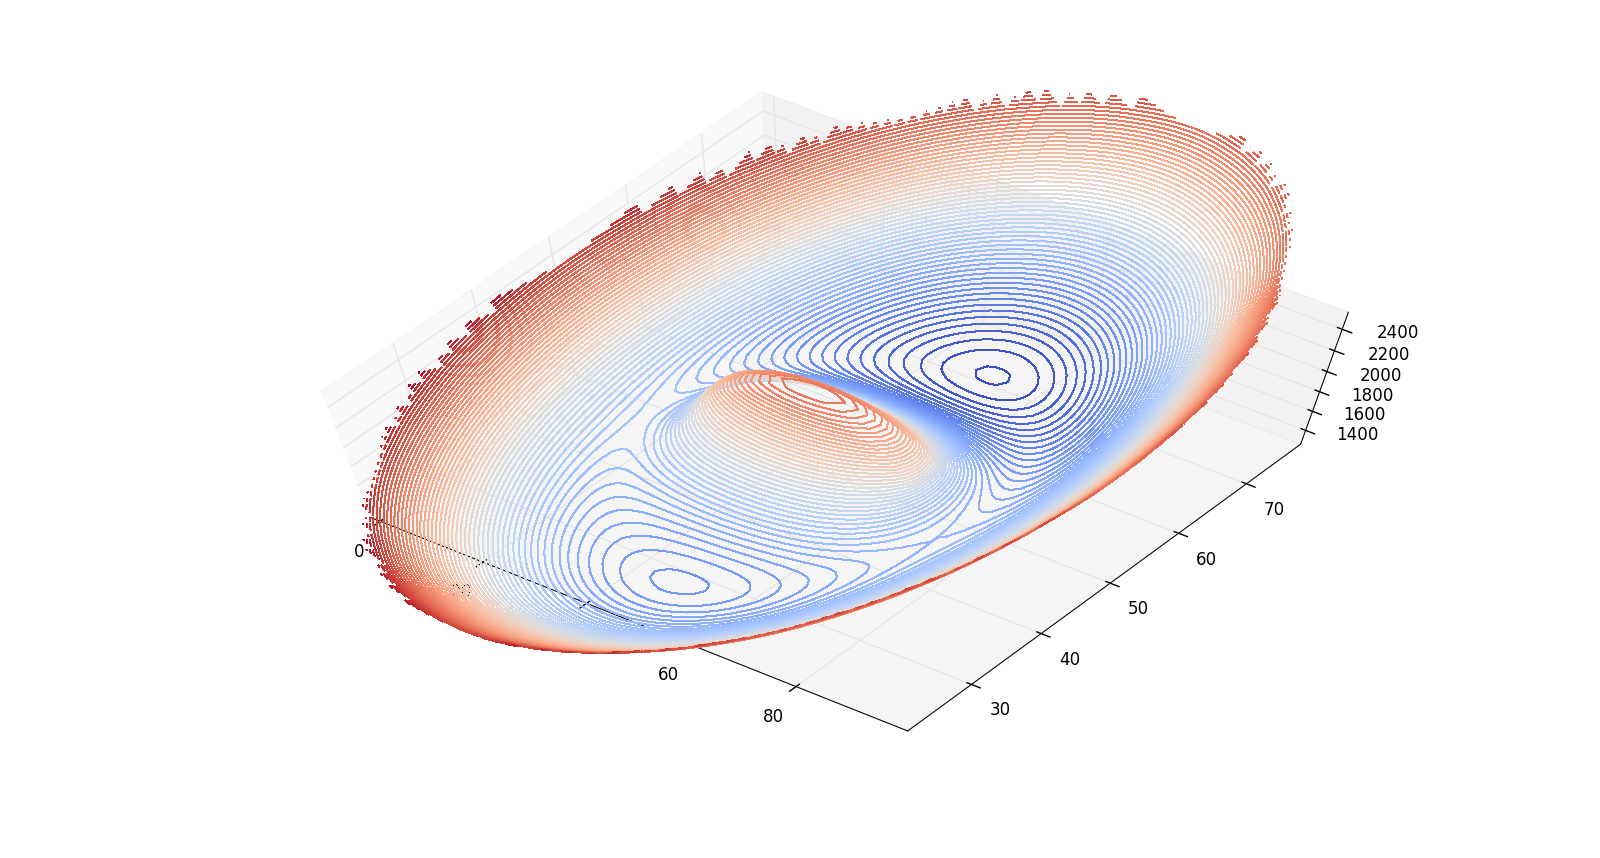
\includegraphics[height=.3\vsize]{fig/arriv3.png}
\caption{Arrival-time surfaces, with contour levels of equal arrival
  time.  The upper surface is with no lens.  The middle surface is
  when a circular lensing mass (offset from the source) is added; a
  maximum, a minimum and a saddle point can be seen.  The last surface
  is the result of an elongated lensing mass; a maximum, two minima
  and two saddle points can be seen.
}
\label{fig:arriv}
\end{figure}

\clearpage

\begin{figure}
  \centering
  \subfigure{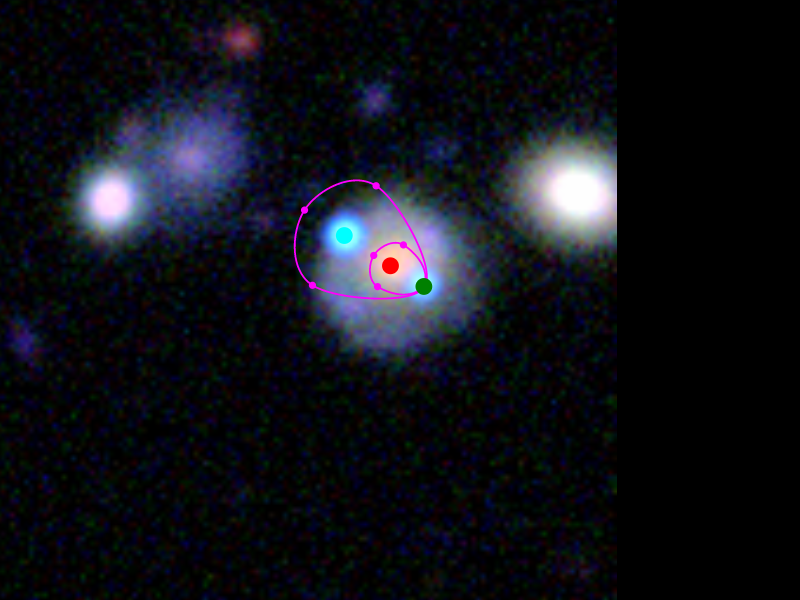
\includegraphics[width=0.45\textwidth]
             {fig/006941_input.png}} \\
  \subfigure{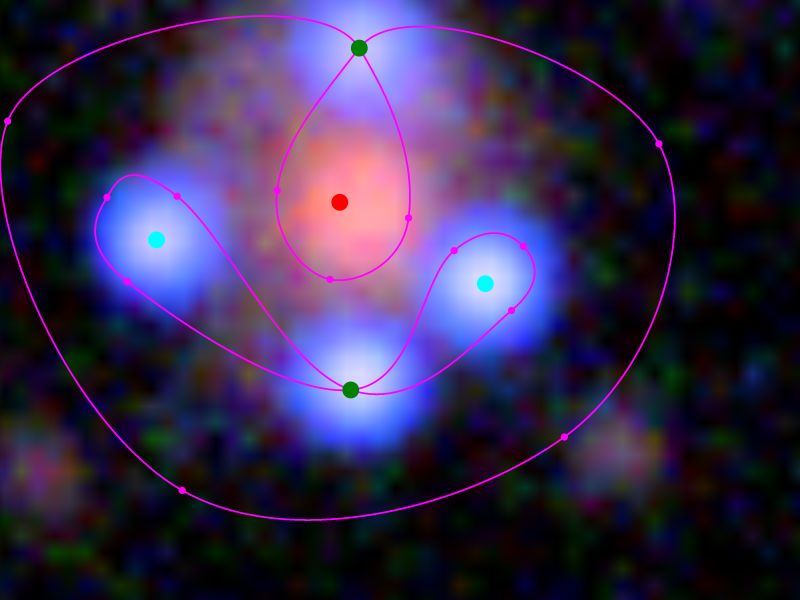
\includegraphics[width=0.45\textwidth]
             {fig/007022_input.png}} \\
  \subfigure{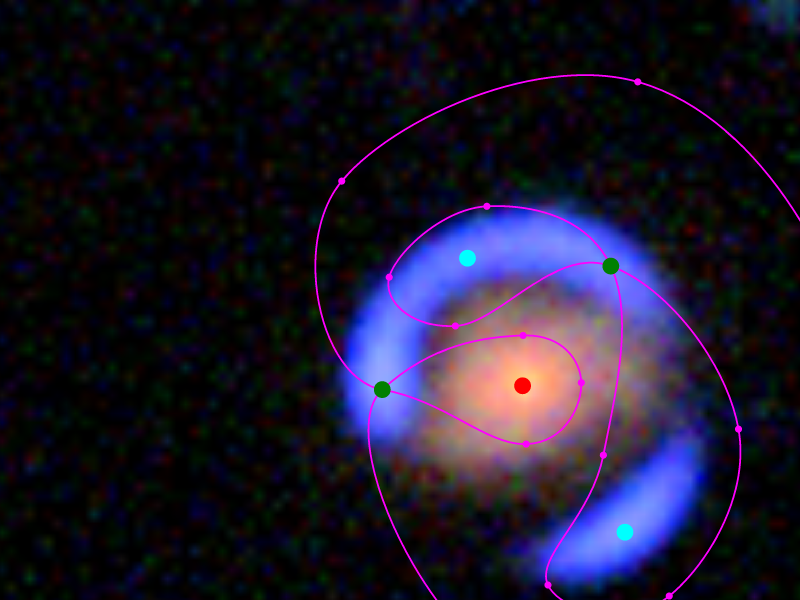
\includegraphics[width=0.45\textwidth]
             {fig/006919_input.png}}
  \caption{Examples of Spaghetti input.  The models from these appear
    later in Figures \ref{fig:6941}, \ref{fig:7022} and \ref{fig:6919}.
  }
  \label{fig:input-spag}
\end{figure}

\clearpage

\begin{figure}
  \centering
  \subfigure[real mass distribution]{
    \label{fig:6941_sim_mass}
    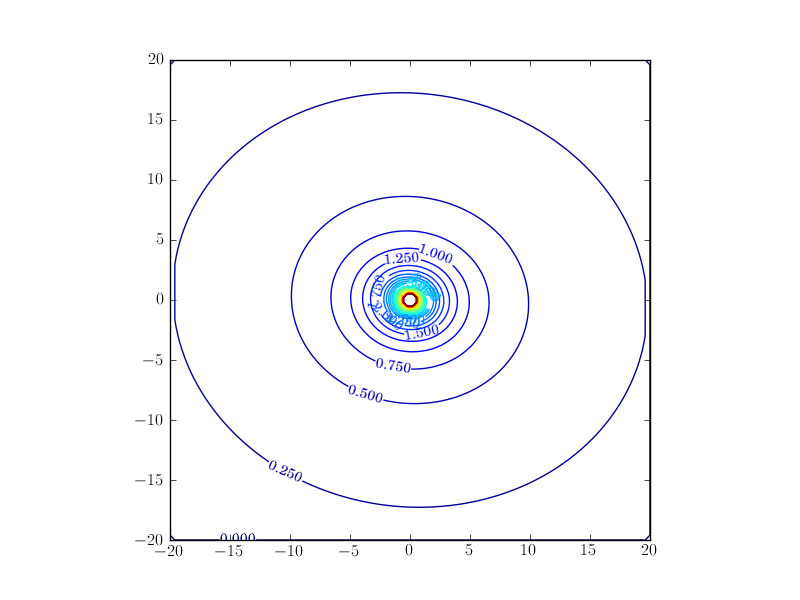
\includegraphics[width=0.45\textwidth]{fig/ASW000102p_kappa.png}
  }
  \subfigure[real arrival-time surface]{
    \label{fig:6941_sim_arr}
    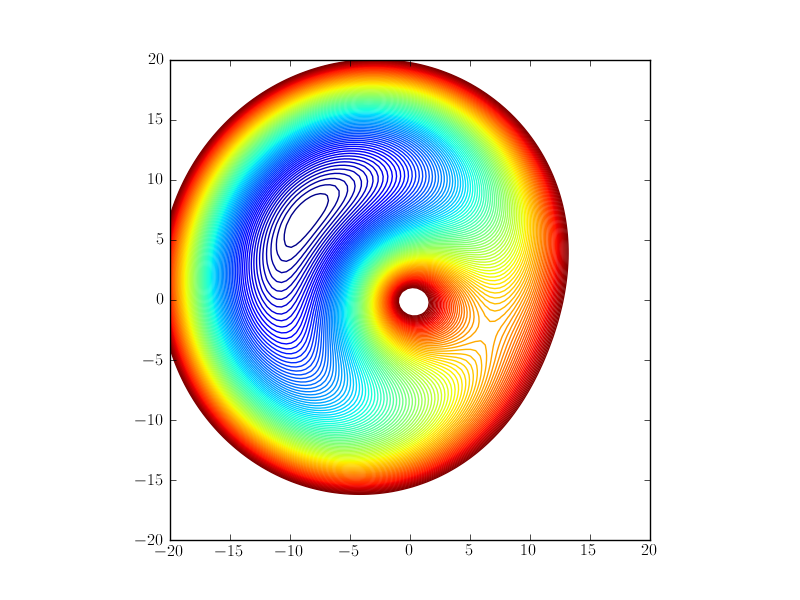
\includegraphics[width=0.45\textwidth]{fig/ASW000102p_arriv.png}
  }
  \subfigure[model mass distribution]{
    \label{fig:6941_mass}
    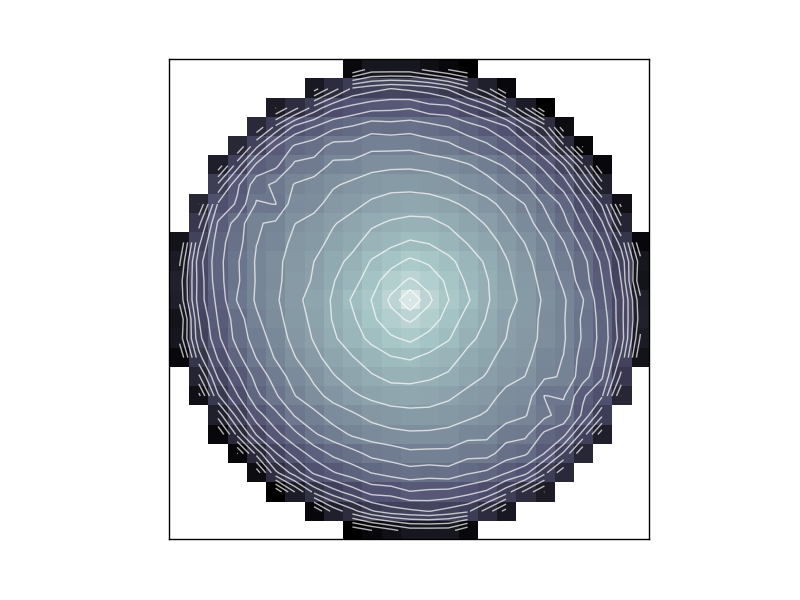
\includegraphics[width=0.45\textwidth]{fig/006941_mass.png}
  }
  \subfigure[model arrival-time surface]{
    \label{fig:6941_cont}
    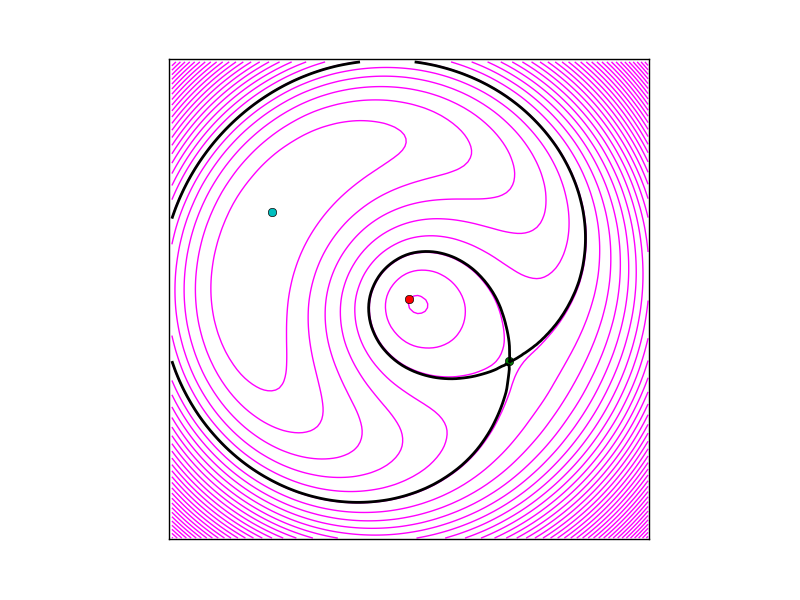
\includegraphics[width=0.45\textwidth]{fig/006941_spaghetti.png}
  }
  \subfigure[real vs model enclosed mass]{
    \label{fig:6941_kappa}
    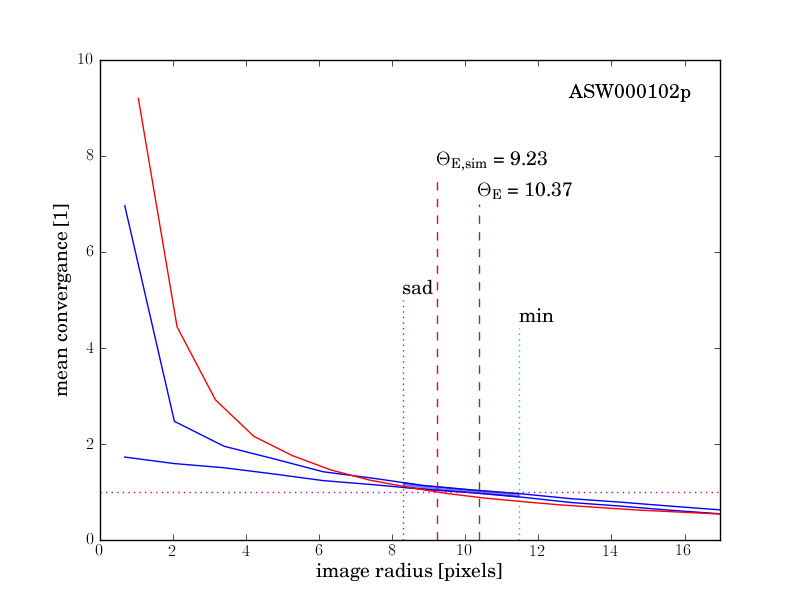
\includegraphics[width=0.45\textwidth]{fig/006941_kappa_encl.png}
  }
  \subfigure[model lensed image]{
    \label{fig:6941_atime}
    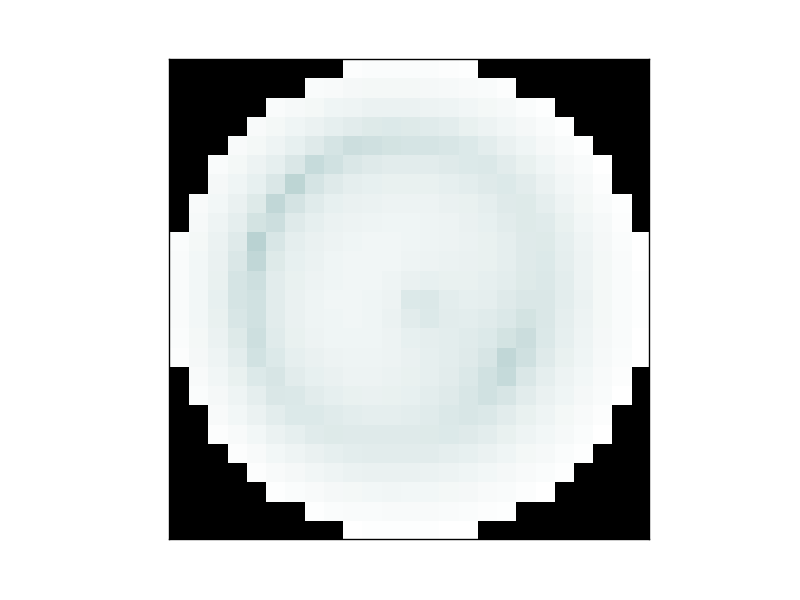
\includegraphics[width=0.45\textwidth]{fig/006941_arr_time.png}
  }
  \caption[result 6941 (ASW000102p)]{Sim ASW000102p and a model.  A
    simple configuration; the model input is shown in the top panel of
    Figure~\ref{fig:input-spag}.  For details of the individual panels
    here, see section \ref{sec:example_models}.}
  \label{fig:6941}
\end{figure}
  
\begin{figure}
  \centering
  \subfigure[real mass distribution]{
    \label{fig:6975_sim_mass}
    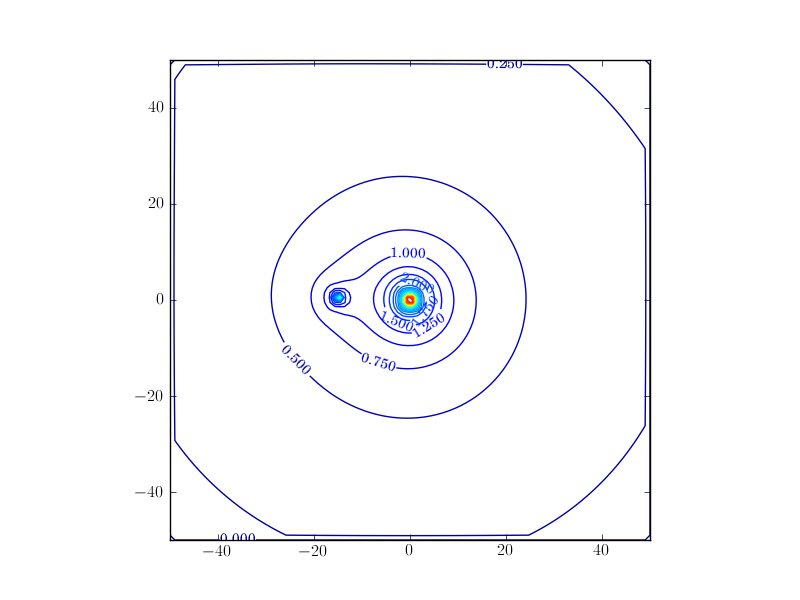
\includegraphics[width=0.45\textwidth]{fig/ASW000195x_kappa.png}
  }
  \subfigure[real arrival-time surface]{
    \label{fig:6975_sim_arr}
    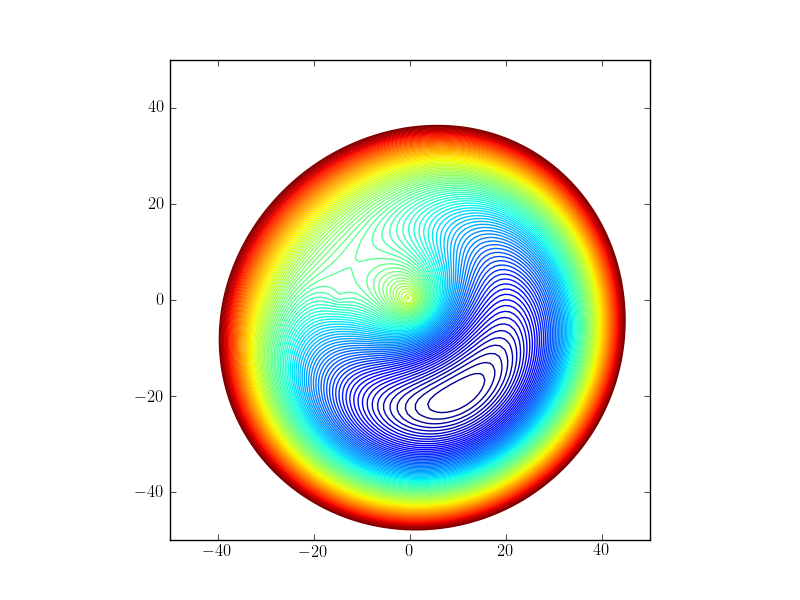
\includegraphics[width=0.45\textwidth]{fig/ASW000195x_arriv.png}
  }
  \subfigure[model mass distribution]{
    \label{fig:6975_mass}
    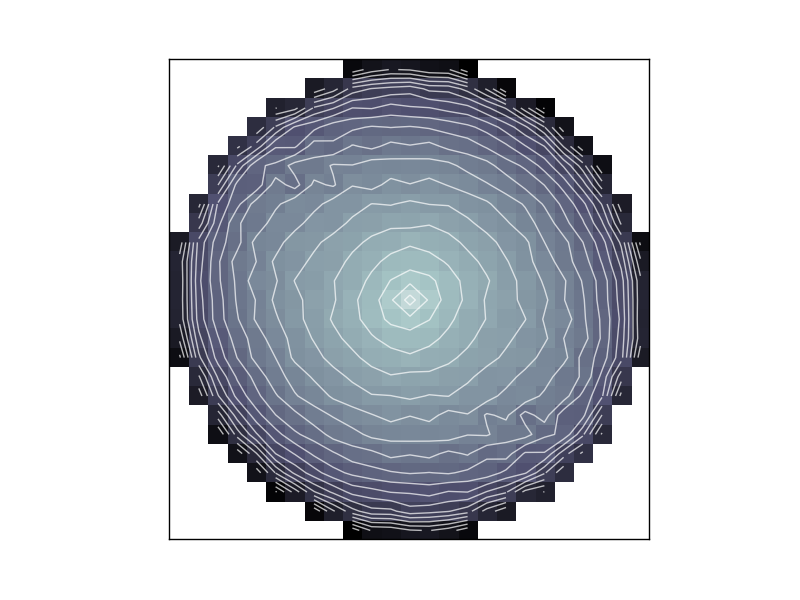
\includegraphics[width=0.45\textwidth]{fig/006975_mass.png}
  }
  \subfigure[model arrival-time surface]{
    \label{fig:6975_cont}
    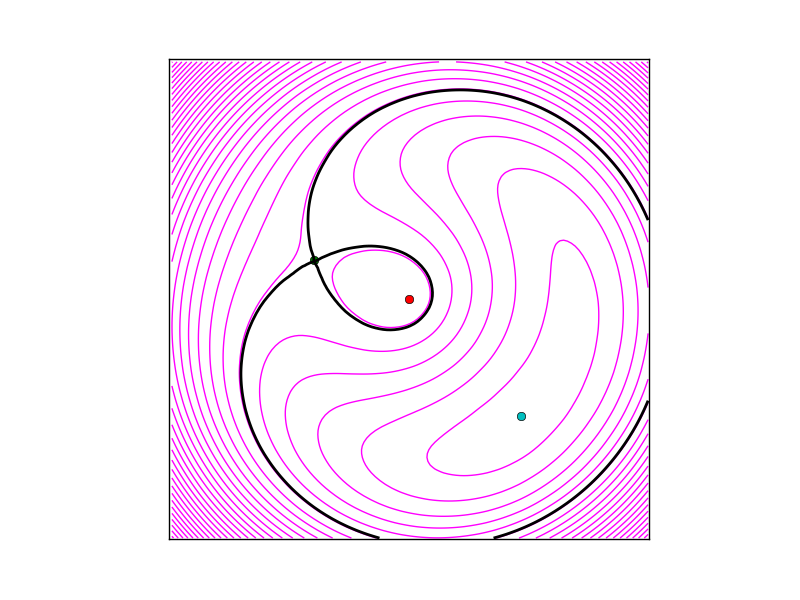
\includegraphics[width=0.45\textwidth]{fig/006975_spaghetti.png}
  }
  \subfigure[real vs model enclosed mass]{
    \label{fig:6975_kappa}
    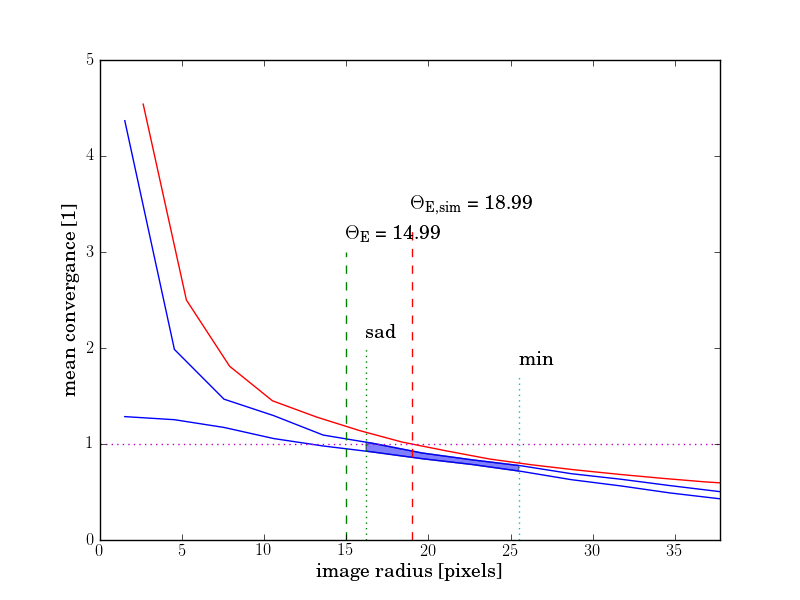
\includegraphics[width=0.45\textwidth]{fig/006975_kappa_encl.png}
  }
  \subfigure[model lensed image]{
    \label{fig:6975_atime}
    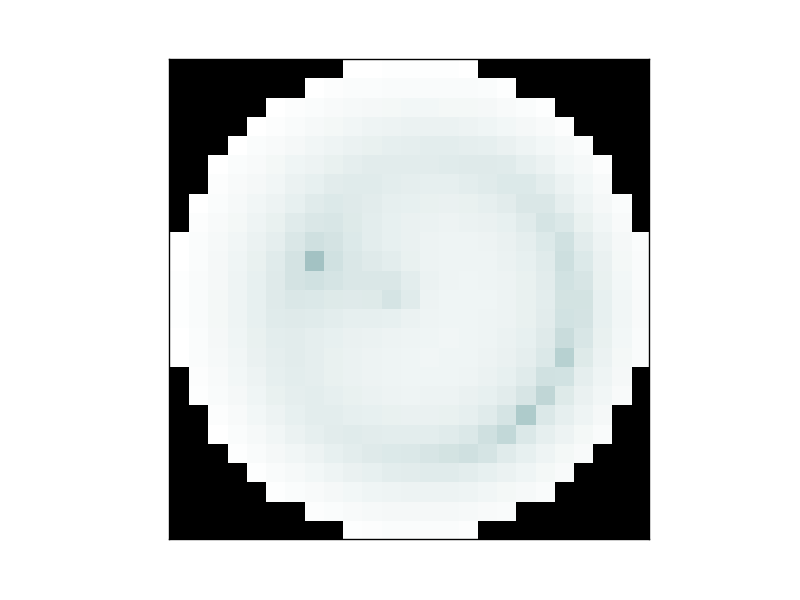
\includegraphics[width=0.45\textwidth]{fig/006975_arr_time.png}
  }
  \caption[result 6975 (ASW000195x)]{Sim ASW000195x and a
    model.}
  \label{fig:6975}
\end{figure}
  
\begin{figure}
  \centering
  \subfigure[real mass distribution]{
    \label{fig:6937_sim_mass}
    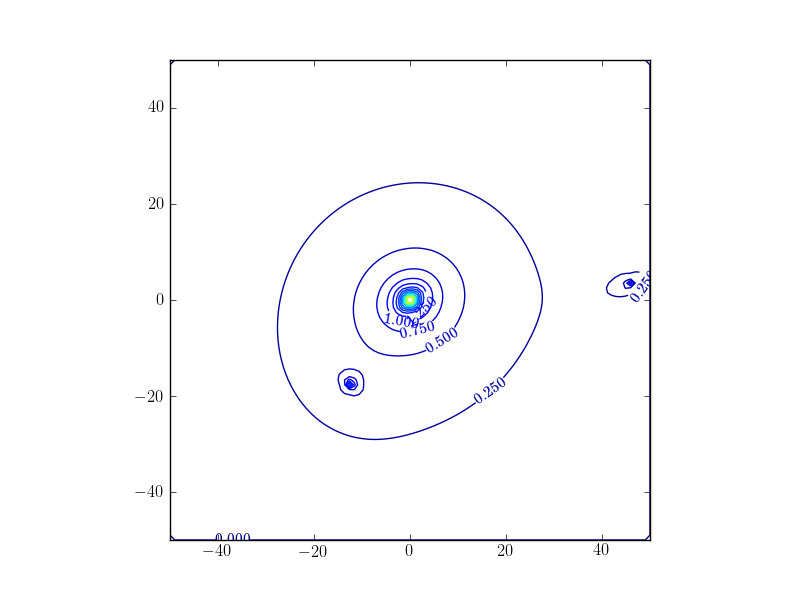
\includegraphics[width=0.45\textwidth]{fig/ASW0000vqg_kappa.png}
  }
  \subfigure[real arrival-time surface]{
    \label{fig:6937_sim_arr}
    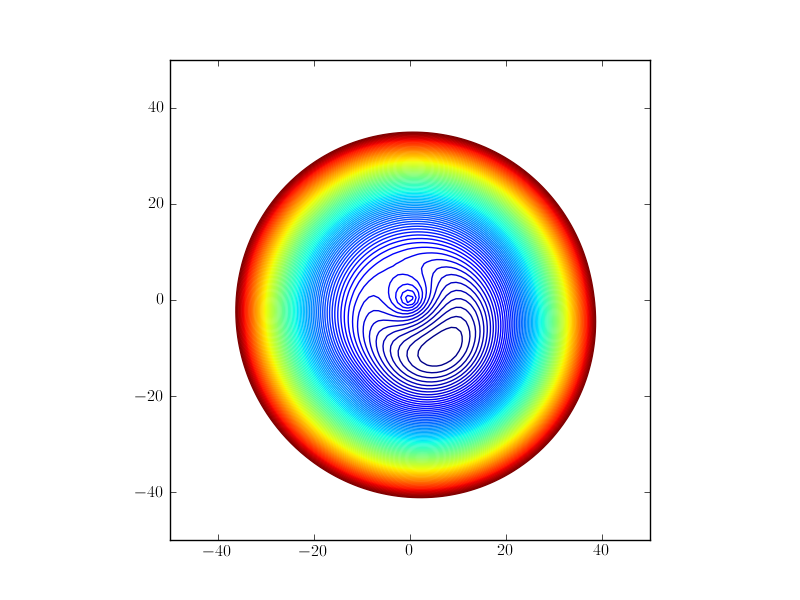
\includegraphics[width=0.45\textwidth]{fig/ASW0000vqg_arriv.png}
  }
  \subfigure[model mass distribution]{
    \label{fig:6937_mass}
    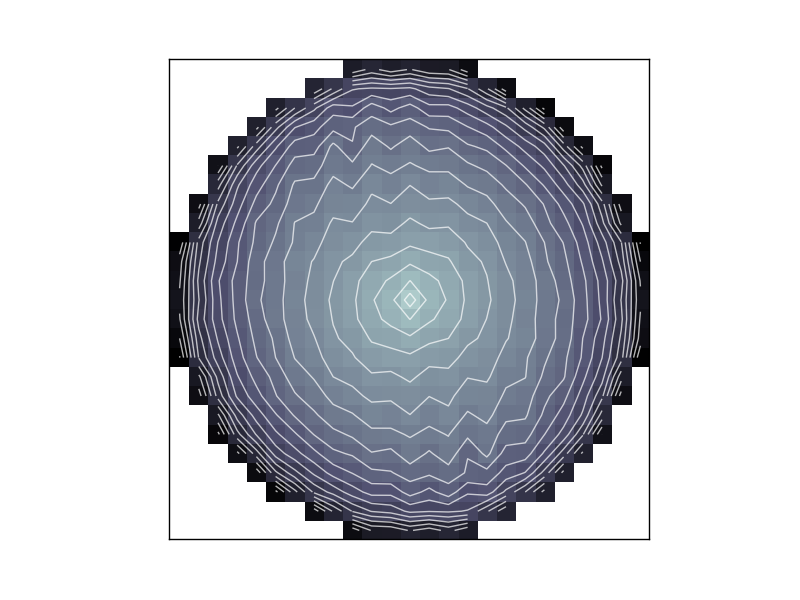
\includegraphics[width=0.45\textwidth]{fig/006937_mass.png}
  }
  \subfigure[model arrival-time surface]{
    \label{fig:6937_cont}
    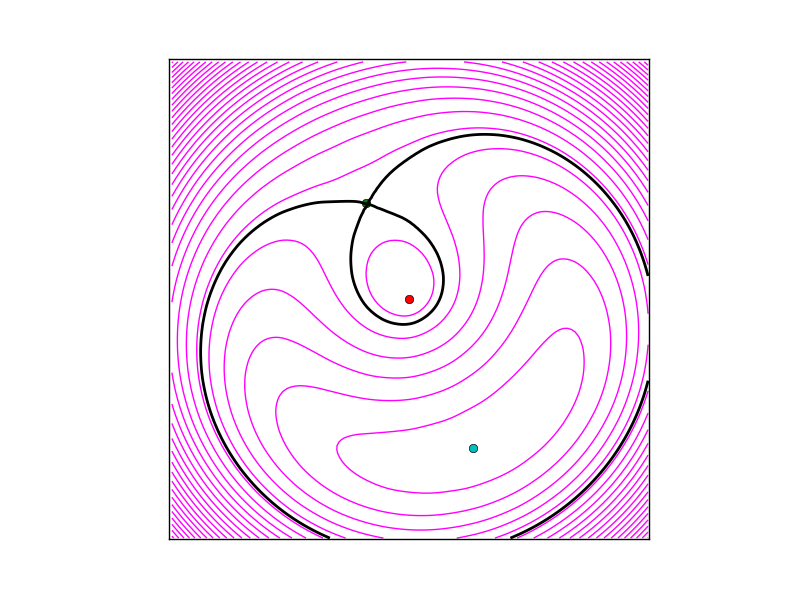
\includegraphics[width=0.45\textwidth]{fig/006937_spaghetti.png}
  }
  \subfigure[real vs model enclosed mass]{
    \label{fig:6937_kappa}
    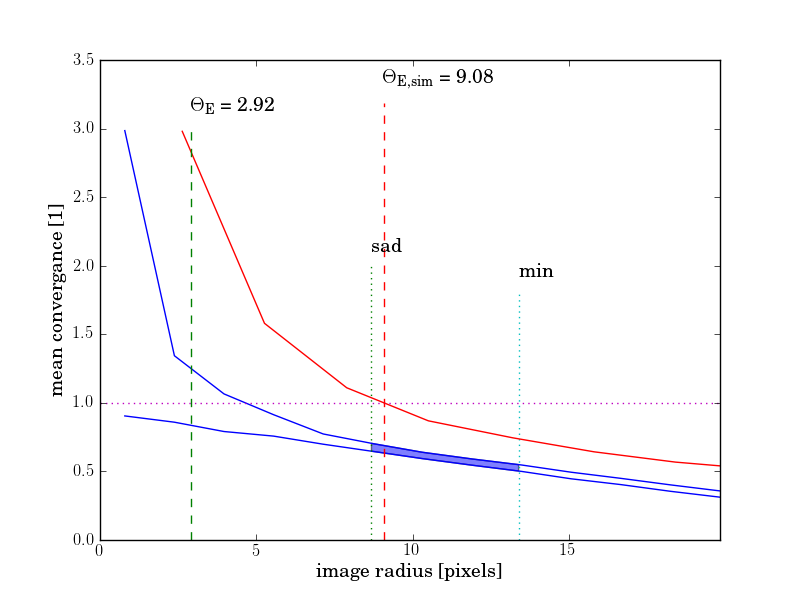
\includegraphics[width=0.45\textwidth]{fig/006937_kappa_encl.png}
  }
  \subfigure[model lensed image]{
    \label{fig:6937_atime}
    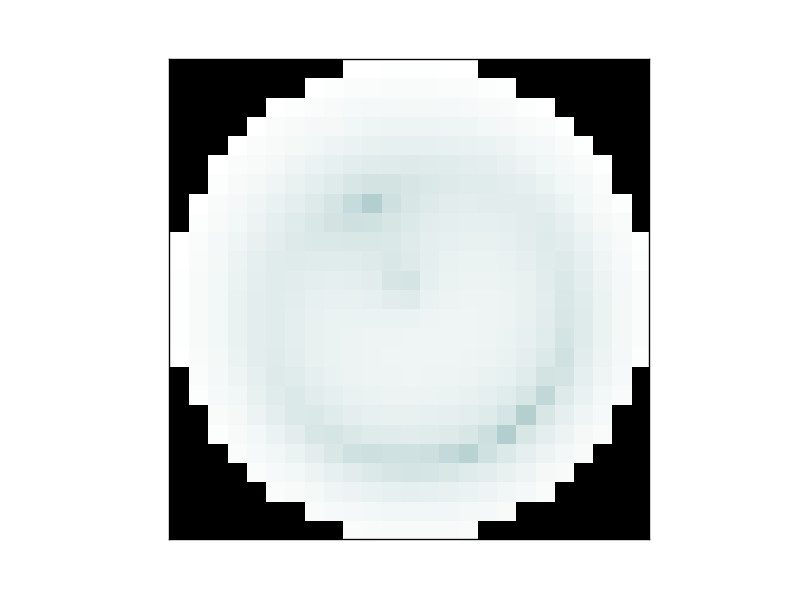
\includegraphics[width=0.45\textwidth]{fig/006937_arr_time.png}
  }
  \caption[result 6937 (ASW0000vqg)]{Sim ASW0000vqg and a model.}
  \label{fig:6937}
\end{figure}

\begin{figure}
  \centering
  \subfigure[real mass distribution]{
    \label{fig:6990_sim_mass}
    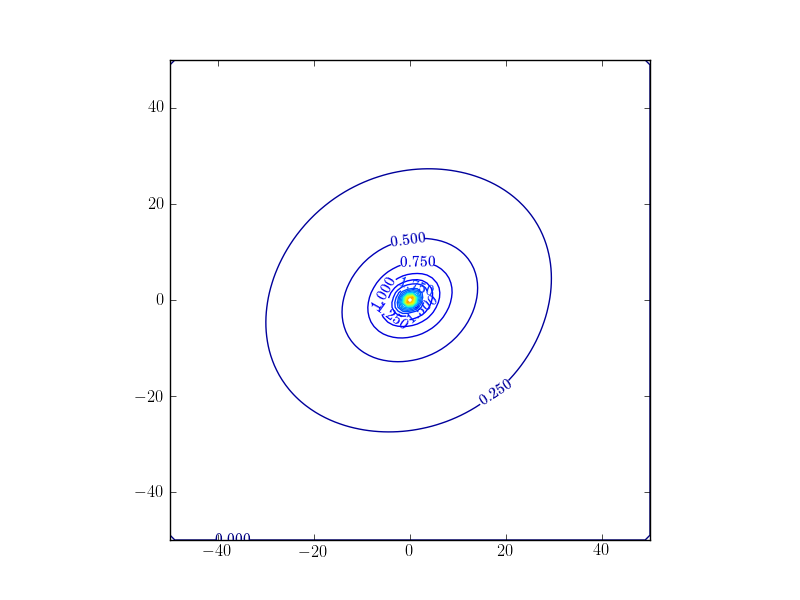
\includegraphics[width=0.45\textwidth]{fig/ASW0004oux_kappa.png}
  }
  \subfigure[real arrival-time surface]{
    \label{fig:6990_sim_arr}
    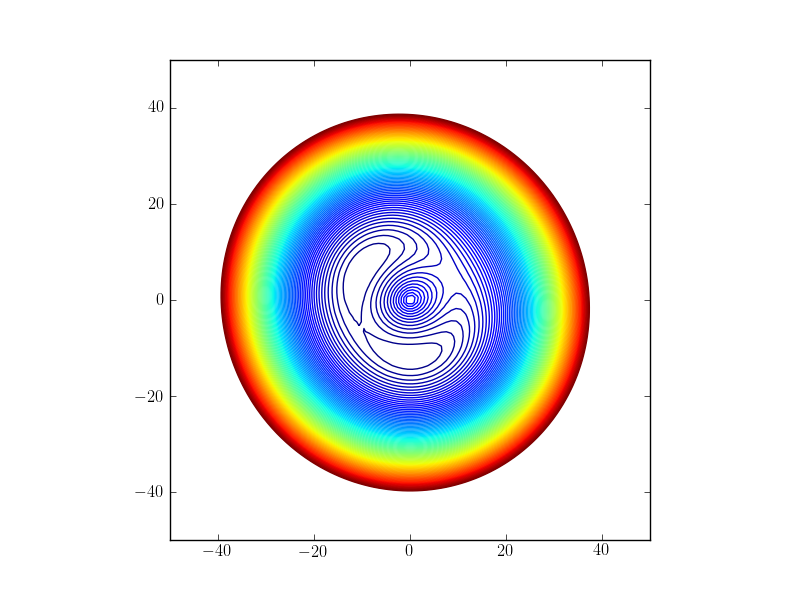
\includegraphics[width=0.45\textwidth]{fig/ASW0004oux_arriv.png}
  }
  \subfigure[model mass distribution]{
    \label{fig:6990_mass}
    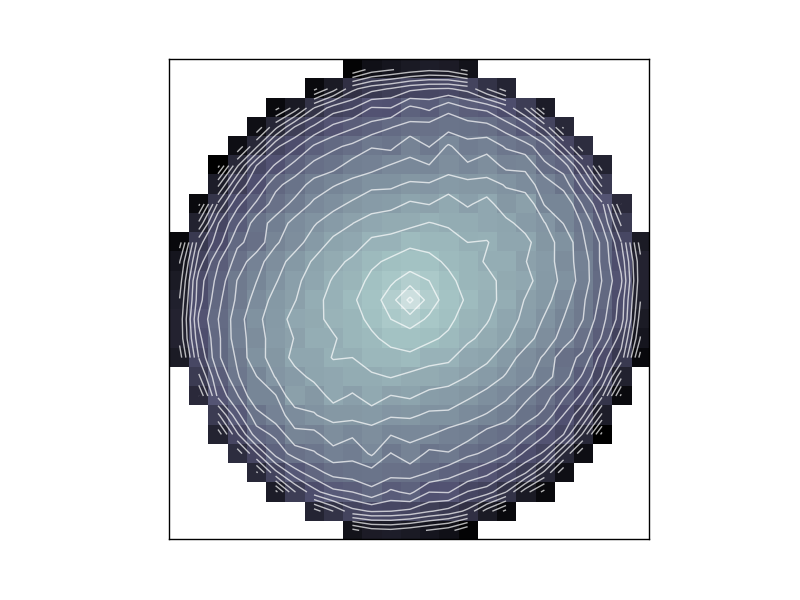
\includegraphics[width=0.45\textwidth]{fig/006990_mass.png}
  }
  \subfigure[model arrival-time surface]{
    \label{fig:6990_cont}
    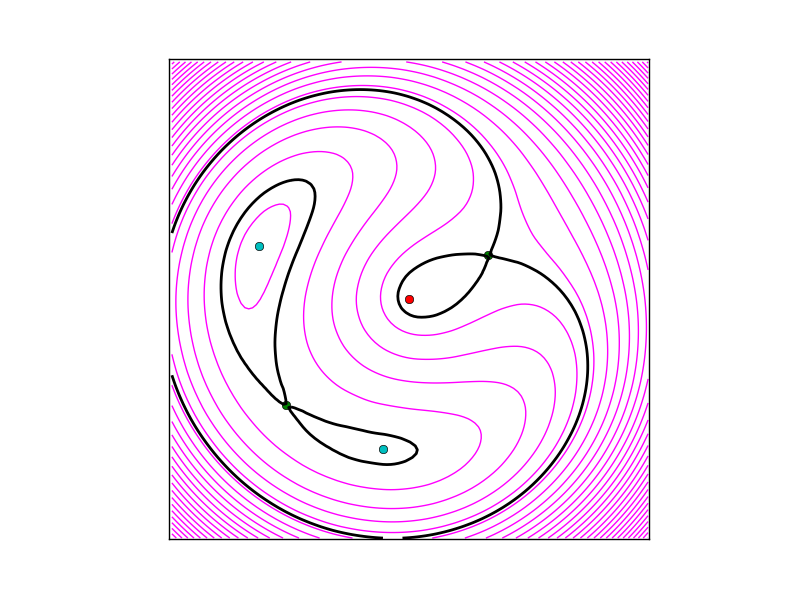
\includegraphics[width=0.45\textwidth]{fig/006990_spaghetti.png}
  }
  \subfigure[real vs model enclosed mass]{
    \label{fig:6990_kappa}
    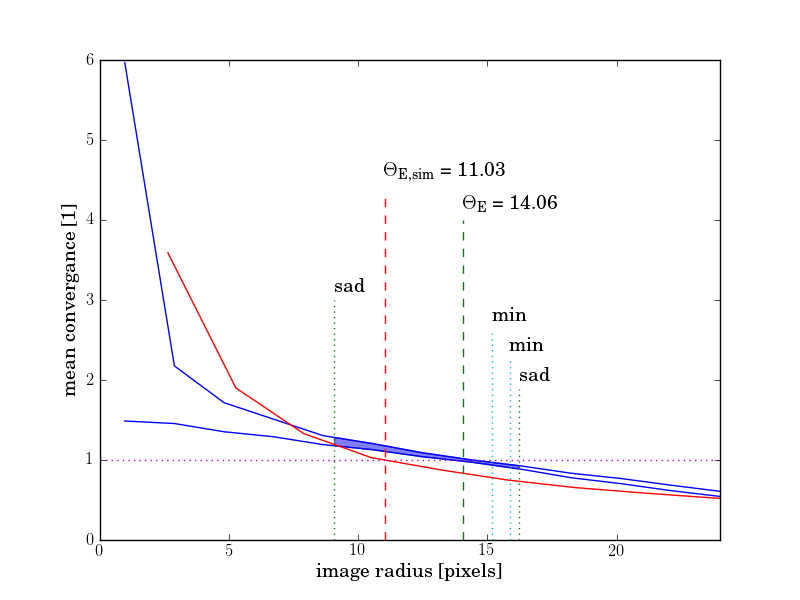
\includegraphics[width=0.45\textwidth]{fig/006990_kappa_encl.png}
  }
  \subfigure[model lensed image]{
    \label{fig:6990_atime}
    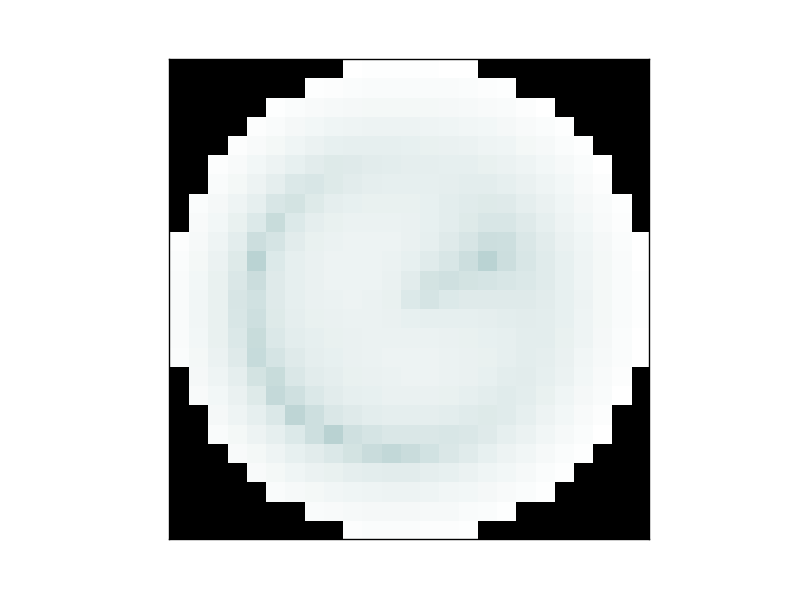
\includegraphics[width=0.45\textwidth]{fig/006990_arr_time.png}
  }

  \caption[result 6990 (ASW0004oux)]{Sim ASW0004oux and a model.}
  \label{fig:6990}
\end{figure}

\begin{figure}
  \centering
  \subfigure[real mass distribution]{
    \label{fig:6915_sim_mass}
    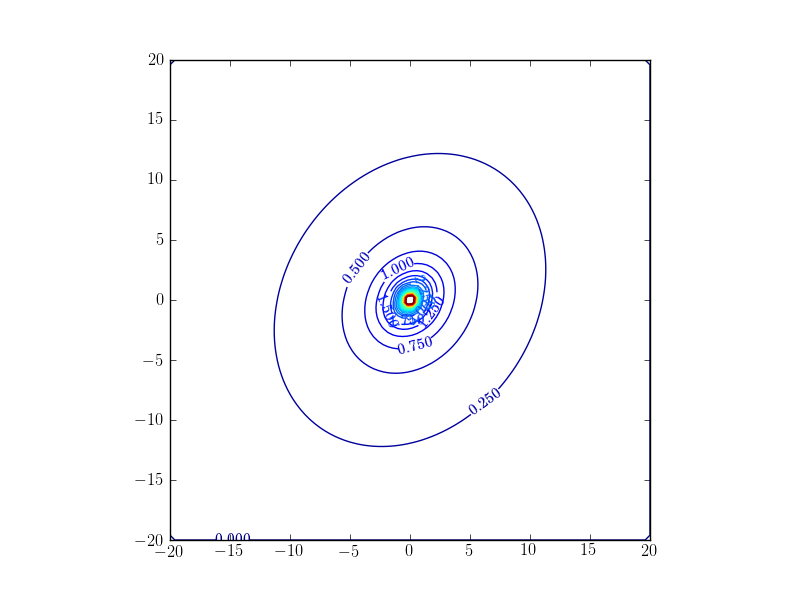
\includegraphics[width=0.45\textwidth]{fig/ASW0001hpf_kappa.png}
  }
  \subfigure[real arrival-time surface]{
    \label{fig:6915_sim_arr}
    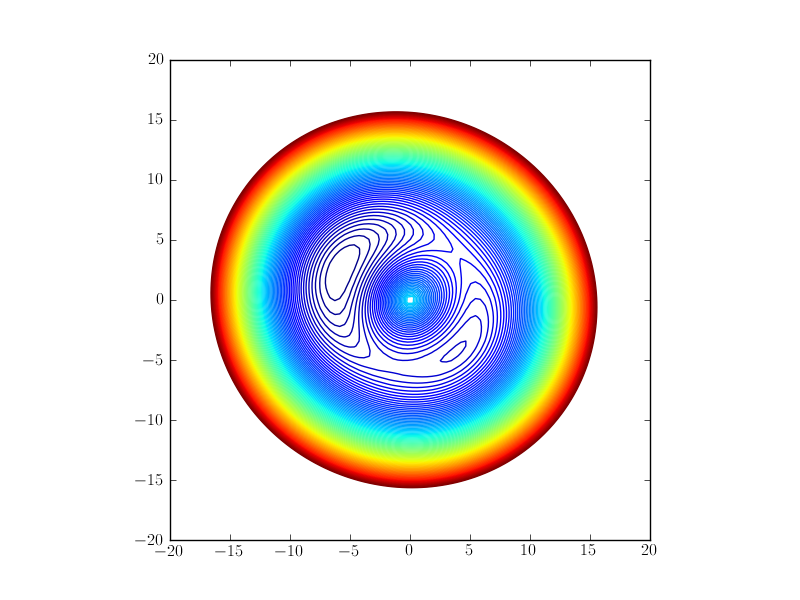
\includegraphics[width=0.45\textwidth]{fig/ASW0001hpf_arriv.png}
  }
  \subfigure[model mass distribution]{
    \label{fig:6915_mass}
    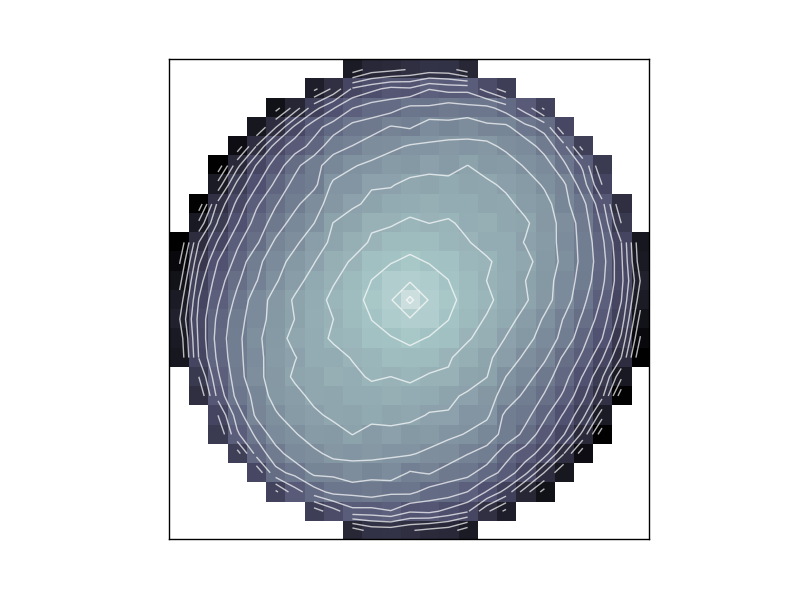
\includegraphics[width=0.45\textwidth]{fig/006915_mass.png}
  }
  \subfigure[model arrival-time surface]{
    \label{fig:6915_cont}
    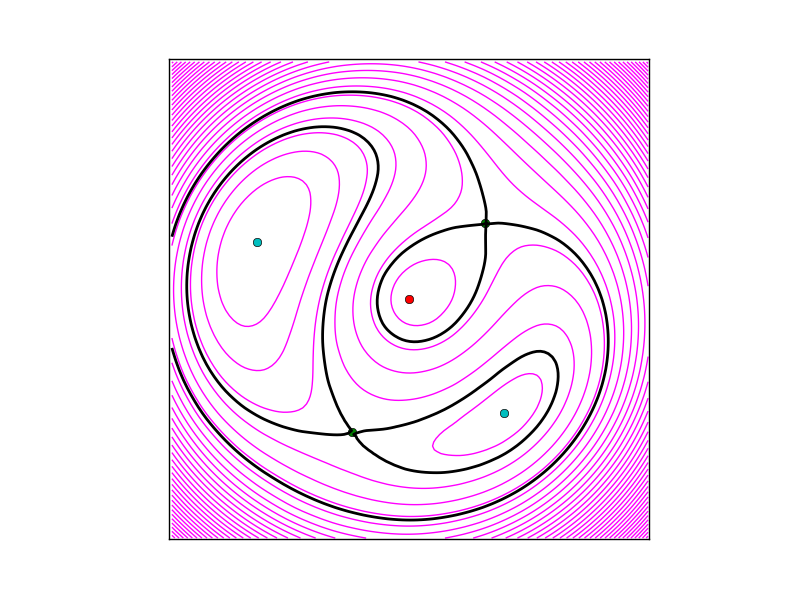
\includegraphics[width=0.45\textwidth]{fig/006915_spaghetti.png}
  }
  \subfigure[real vs model enclosed mass]{
    \label{fig:6915_kappa}
    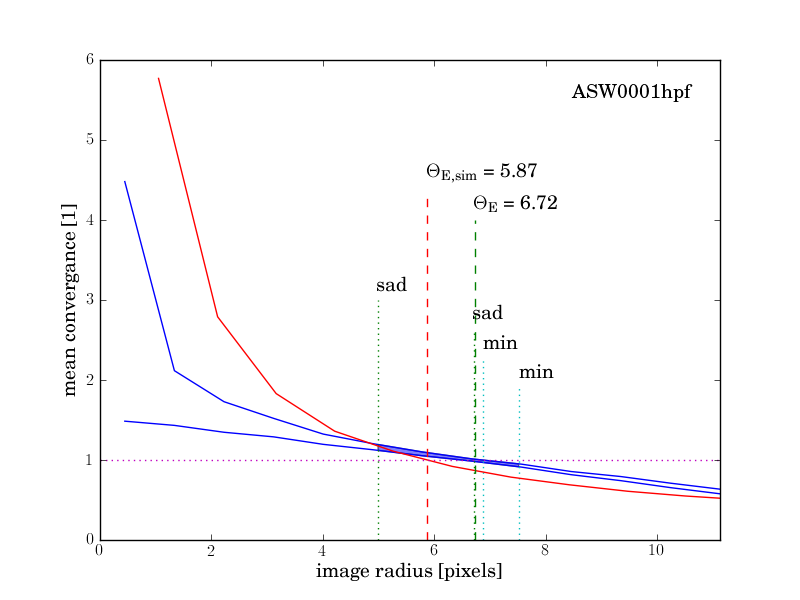
\includegraphics[width=0.45\textwidth]{fig/006915_kappa_encl.png}
  }
  \subfigure[model lensed image]{
    \label{fig:6915_atime}
    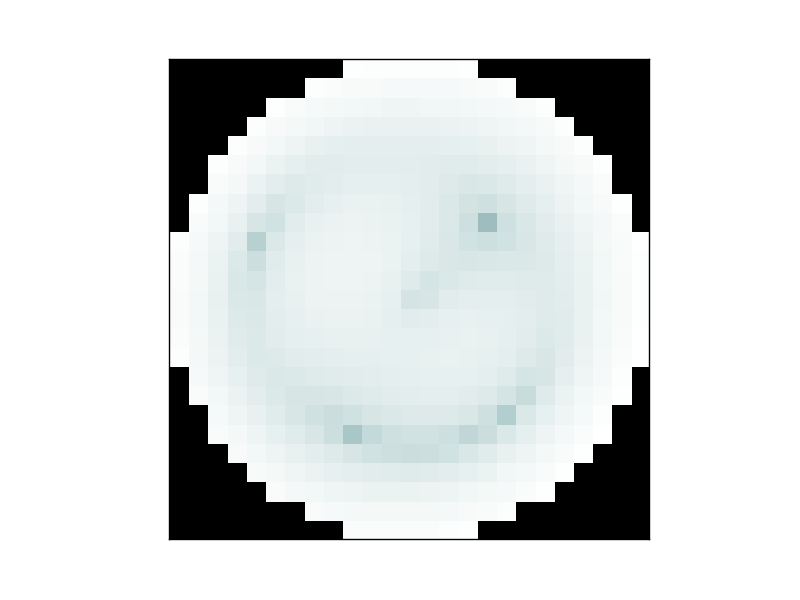
\includegraphics[width=0.45\textwidth]{fig/006915_arr_time.png}
  }

  \caption[result 6915 (ASW0001hpf)]{Sim ASW0001hpf and a model. Inclined quad.}
  \label{fig:6915}
\end{figure}

  
\begin{figure}
  \centering
  \subfigure[real mass distribution]{
    \label{fig:7022_sim_mass}
    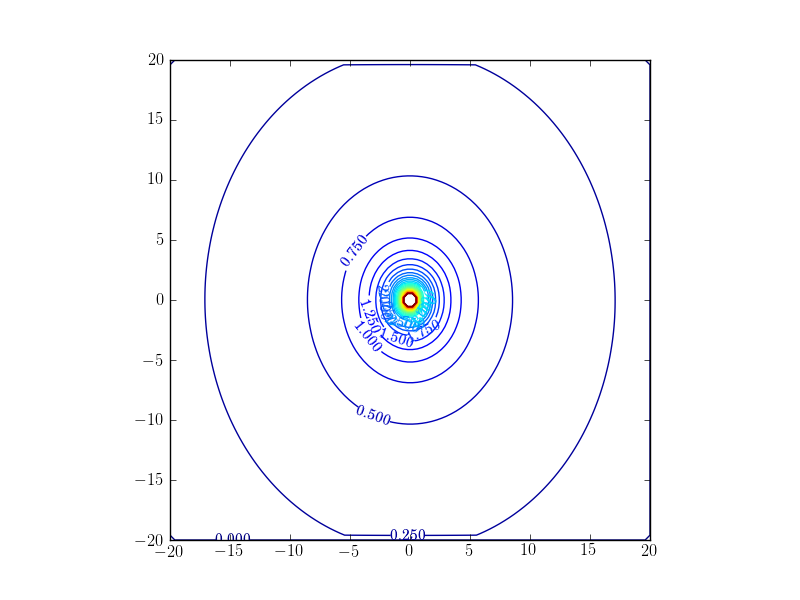
\includegraphics[width=0.45\textwidth]{fig/ASW0000h2m_kappa.png}
  }
  \subfigure[real arrival-time surface]{
    \label{fig:7022_sim_arr}
    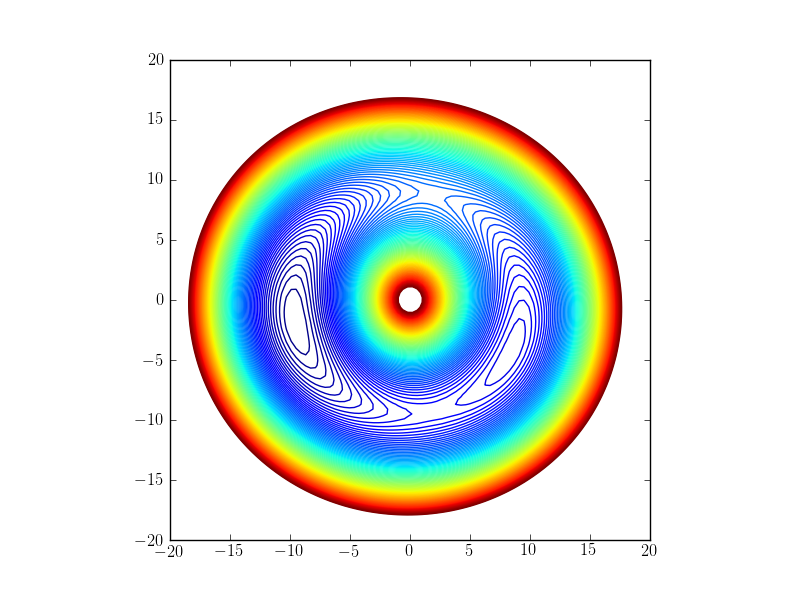
\includegraphics[width=0.45\textwidth]{fig/ASW0000h2m_arriv.png}
  }
  \subfigure[model mass distribution]{
    \label{fig:7022_mass}
    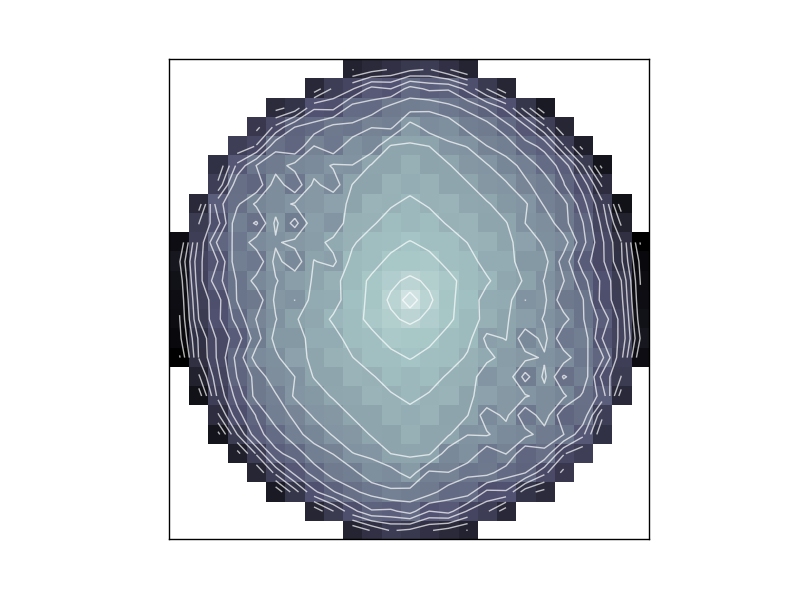
\includegraphics[width=0.45\textwidth]{fig/007022_mass.png}
  }
  \subfigure[model arrival-time surface]{
    \label{fig:7022_cont}
    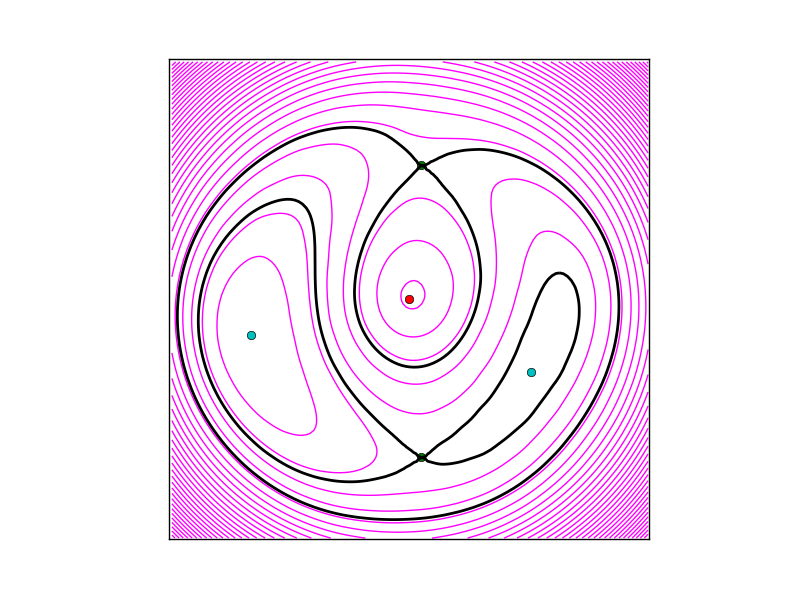
\includegraphics[width=0.45\textwidth]{fig/007022_spaghetti.png}
  }
  \subfigure[real vs model enclosed mass]{
    \label{fig:7022_kappa}
    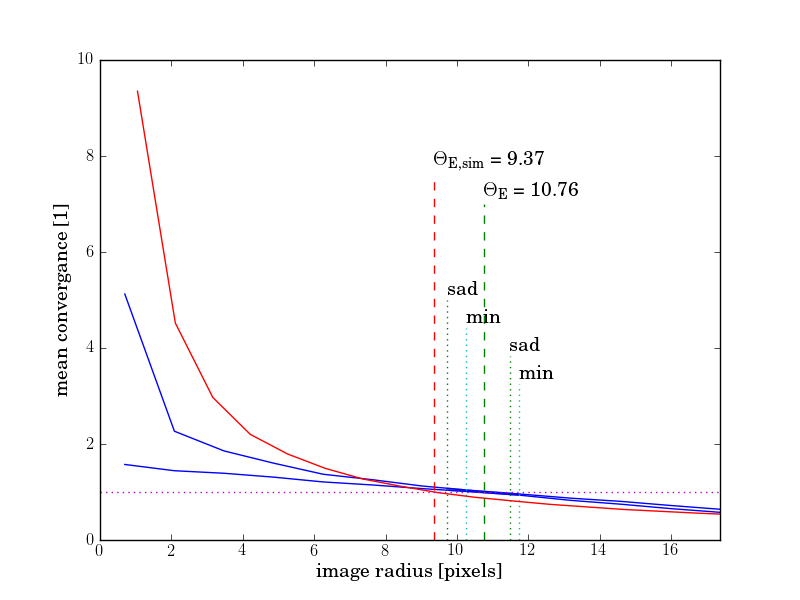
\includegraphics[width=0.45\textwidth]{fig/007022_kappa_encl.png}
  }
  \subfigure[model lensed image]{
    \label{fig:7022_atime}
    \includegraphics[width=0.45\textwidth]{fig/007022_arr_time.png}
  }

  \caption[result 7022 (ASW0000h2m)]{Sim ASW0000h2m and a model.  The
    model input appears in the middle panel of Figure
    \ref{fig:input-spag}.}
  \label{fig:7022}
\end{figure}
  
\begin{figure}
  \centering
  \subfigure[real mass distribution]{
    \label{fig:7025_sim_mass}
    \includegraphics[width=0.45\textwidth]{fig/ASW0000h2m_kappa.png}
  }
  \subfigure[real arrival-time surface]{
    \label{fig:7025_sim_arr}
    \includegraphics[width=0.45\textwidth]{fig/ASW0000h2m_arriv.png}
  }
  \subfigure[model mass distribution]{
    \label{fig:7025_mass}
    \includegraphics[width=0.45\textwidth]{fig/007025_mass.png}
  }
  \subfigure[model arrival-time surface]{
    \label{fig:7025_cont}
    \includegraphics[width=0.45\textwidth]{fig/007025_spaghetti.png}
  }
  \subfigure[real vs model enclosed mass]{
    \label{fig:7025_kappa}
    \includegraphics[width=0.45\textwidth]{fig/007025_kappa_encl.png}
  }
  \subfigure[model lensed image]{
    \label{fig:7025_atime}
    \includegraphics[width=0.45\textwidth]{fig/007025_arr_time.png}
  }

  \caption[result 7025 (ASW0000h2m)]{Sim ASW0000h2m and another model.  The image parities in this case were incorrectly identified.}
  \label{fig:7025}
\end{figure}
  

\begin{figure}
  \centering
  \subfigure[real mass distribution]{
    \label{fig:6919_sim_mass}
    \includegraphics[width=0.45\textwidth]{fig/ASW0002z6f_kappa.png}
  }
  \subfigure[real arrival-time surface]{
    \label{fig:6919_sim_arr}
    \includegraphics[width=0.45\textwidth]{fig/ASW0002z6f_arriv.png}
  }
  \subfigure[model mass distribution]{
    \label{fig:6919_mass}
    \includegraphics[width=0.45\textwidth]{fig/006919_mass.png}
  }
  \subfigure[model arrival-time surface]{
    \label{fig:6919_cont}
    \includegraphics[width=0.45\textwidth]{fig/006919_spaghetti.png}
  }
  \subfigure[real vs model enclosed mass]{
    \label{fig:6919_kappa}
    \includegraphics[width=0.45\textwidth]{fig/006919_kappa_encl.png}
  }
  \subfigure[model lensed image]{
    \label{fig:6919_atime}
    \includegraphics[width=0.45\textwidth]{fig/006919_arr_time.png}
  }
  \caption[result 6919 (ASW0002z6f)]{Sim ASW0002z6f and a model.  The
    model input appears in the bottom panel of Figure
    \ref{fig:input-spag}. An incipient quad}
  \label{fig:6919}
\end{figure}


\clearpage

\begin{figure}[htbp]
  \centering
    \includegraphics[width=0.80\textwidth]{fig/eR_1.png}
  \caption{\ERf for all models with estimated errors in blue squares, \ERg of simulation in red crosses}
  \label{fig:ER_all_models}
\end{figure}

\begin{figure}[htbp]
  \centering
    \includegraphics[width=0.80\textwidth]{fig/eR_4.png}
  \caption{Relative \ERf / \ERg[, sim] for models by volunteers (blue cross), models made by an expert (red cross with offset), including rejected models (green squares); binned per sim.}
  \label{fig:ER_per_sim}
\end{figure}

\begin{figure}
  \centering
  \subfigure{\includegraphics[width=0.45\textwidth]
             {fig/007020_kappa_encl}}
  \subfigure{\includegraphics[width=0.45\textwidth]
             {fig/007021_kappa_encl}} \\
  \subfigure{\includegraphics[width=0.45\textwidth]
             {fig/007024_kappa_encl}}
  \subfigure{\includegraphics[width=0.45\textwidth]
             {fig/007025_kappa_encl}}
  \subfigure{\includegraphics[width=0.45\textwidth]
             {fig/007022_kappa_encl}}
  \caption{\kenc for models of \asw{0h2m}: 7020 (top left), 7021 (top right), 7024 (mid left), 7025 (mid right) by volunteers and a correct model 7022 (bottom) by an expert.}
  \label{fig:kapenc_compare_faulty}
\end{figure}



\newpage

%\listoftodos

\end{document}

